%% Overleaf			
%% Software Manual and Technical Document Template	
%% 									
%% This provides an example of a software manual created in Overleaf.

\documentclass{tower-manual}

\usepackage{draftwatermark}

% Packages used in this example
\usepackage{graphicx}  % for including images
\graphicspath{ {./images} }
\usepackage{microtype} % for typographical enhancements
\usepackage[hidelinks]{hyperref}  % for hyperlinks
\usepackage[a5paper,top=2cm,bottom=2cm,left=1cm,right=1cm]{geometry} % for setting page size and margins
\usepackage{enumitem}
\setlist{itemsep=0.25mm}
\usepackage{lipsum}

\usepackage{caption}
% \DeclareCaptionLabelFormat{simple}
\DeclareCaptionLabelSeparator{none}{}
\captionsetup{labelformat=simple, labelsep=none}

% Custom macros used in this example document
\newcommand{\doclink}[2]{\href{#1}{#2}\footnote{\url{#1}}}
\newcommand{\cs}[1]{\texttt{\textbackslash #1}}

% Frontmatter data; appears on title page
\title{Dani's Indoor Grow Towers \\User Manual}
\author{Rev. 0.0.1}
\date{}
% \author{Overleaf}
% \softwarelogo{\includegraphics[width=8cm]{logo}}

\begin{document}

\pagenumbering{gobble}

\begin{titlepage}
    \maketitle

    \begin{center}
        \begin{minipage}{0.45\textwidth}
            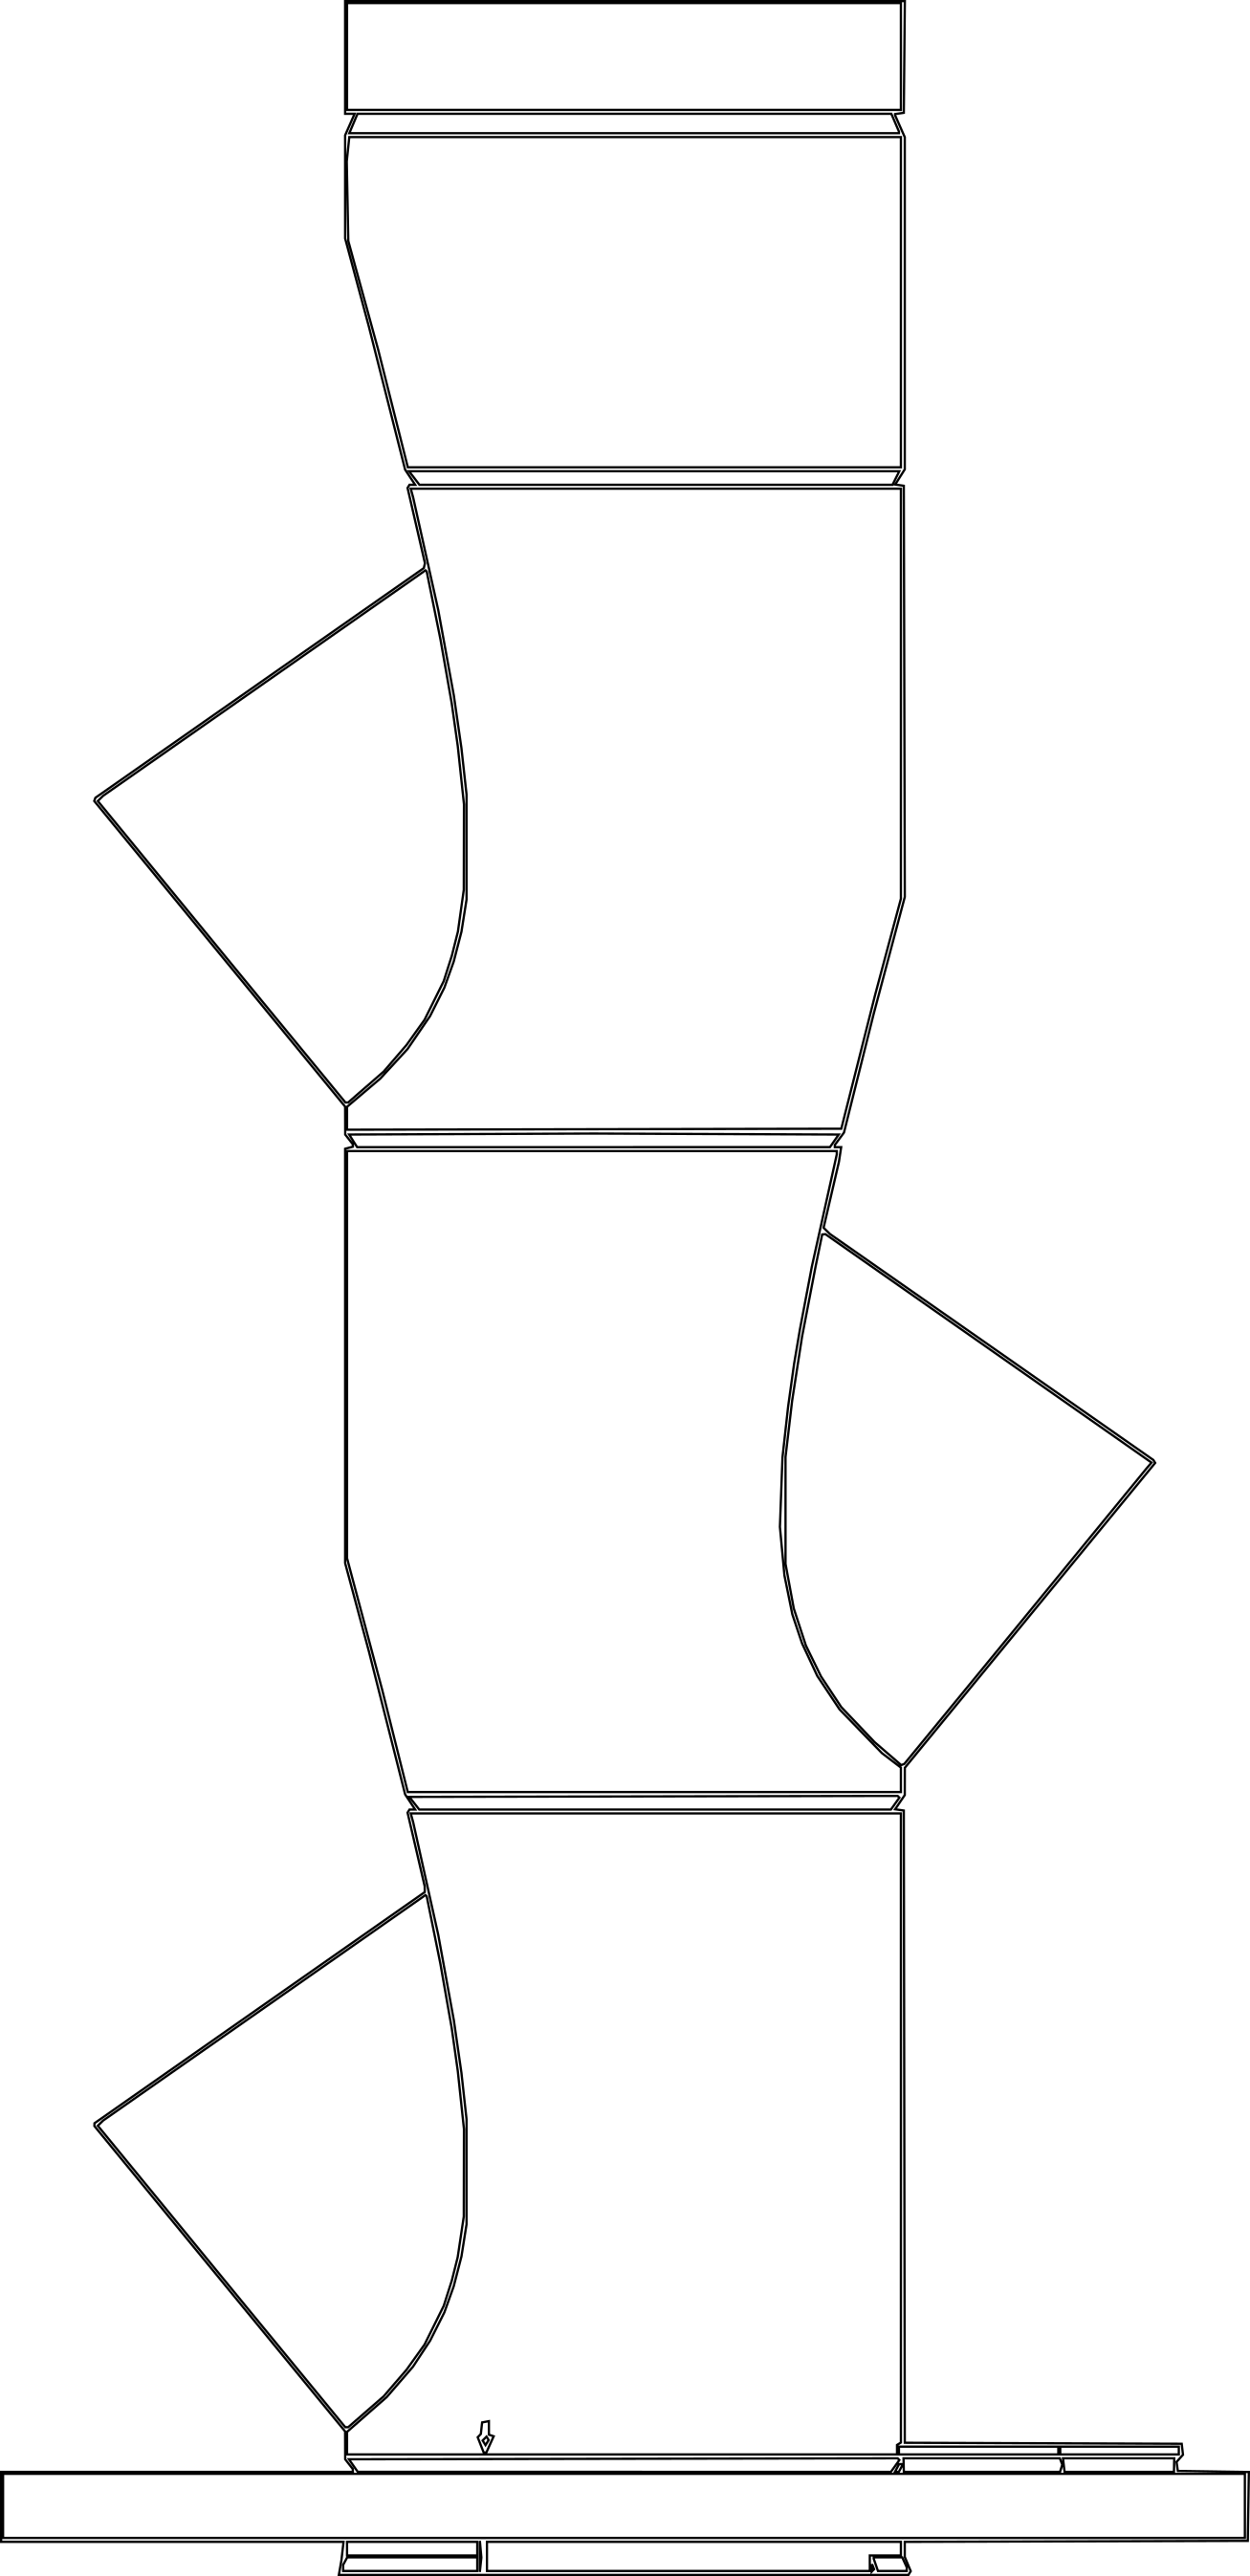
\includegraphics[width=1.0\textwidth]{images/80mm_wireframe.png}
        \end{minipage}
        \hfill
        \begin{minipage}{0.45\textwidth}
            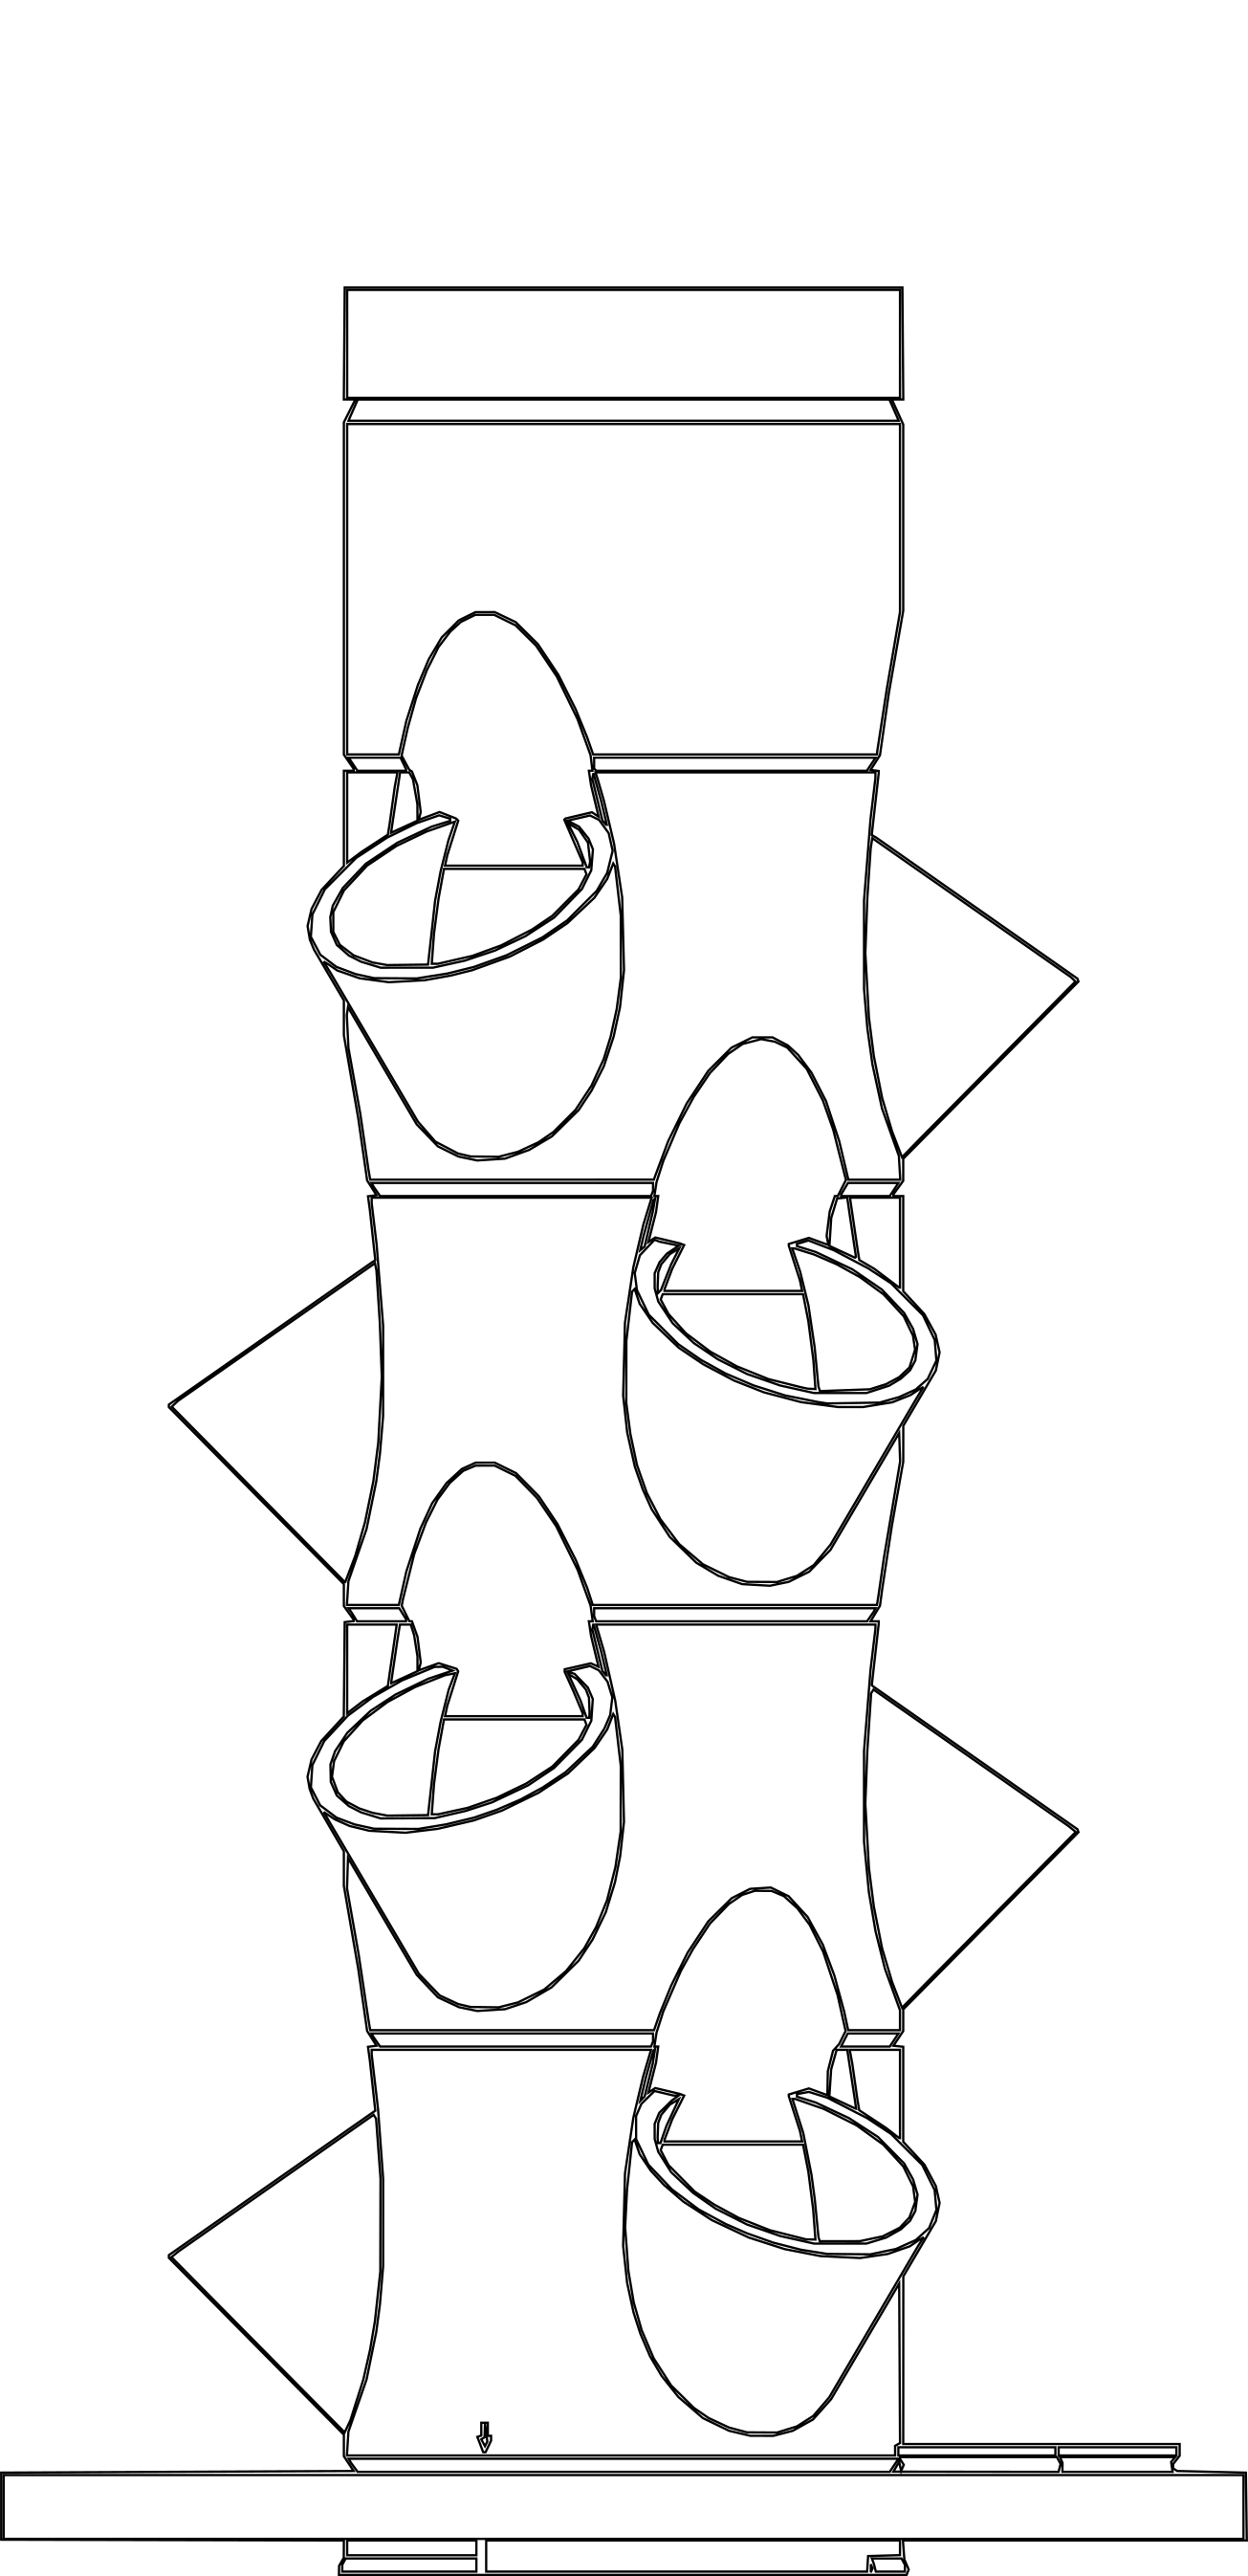
\includegraphics[width=1.0\textwidth]{images/50mm_wireframe.png}
        \end{minipage}
    \end{center}
\end{titlepage}

\blankpage

\tableofcontents

\newpage
\blankpage

\pagenumbering{arabic}

\section{Introduction}

\lipsum[1-2]

\newpage

\section{Precautions}

\begin{itemize}
    \item Proper sanitation is paramount! Ensure your system is cleaned: before and after each growing cycle; if excessive growth of algae, fungus, or biofilm occurs; or if you notice any other signs of bacterial, fungal, algal, or other unwanted contamination. This is to minimize the risk of hazardous pathogens both to your plants \textbf{and} to you.
    \item Remember that your tower is a water vessel. To minimize risk in the event of a spill, place your tower well away from electrical devices, electrical outlets, and any other items which may be damaged by water or which may present a hazard in the presence of water.
    \item The components of your tower are not dishwasher-safe.
    \item Your tower is designed only to be placed indoors. Placing your tower outdoors may result in damage.
\end{itemize}


\newpage

\section{Assembly Instructions -- 80mm}

\subsection{Parts}

\begin{center}
    \begin{minipage}{0.3\textwidth}
        \centering
        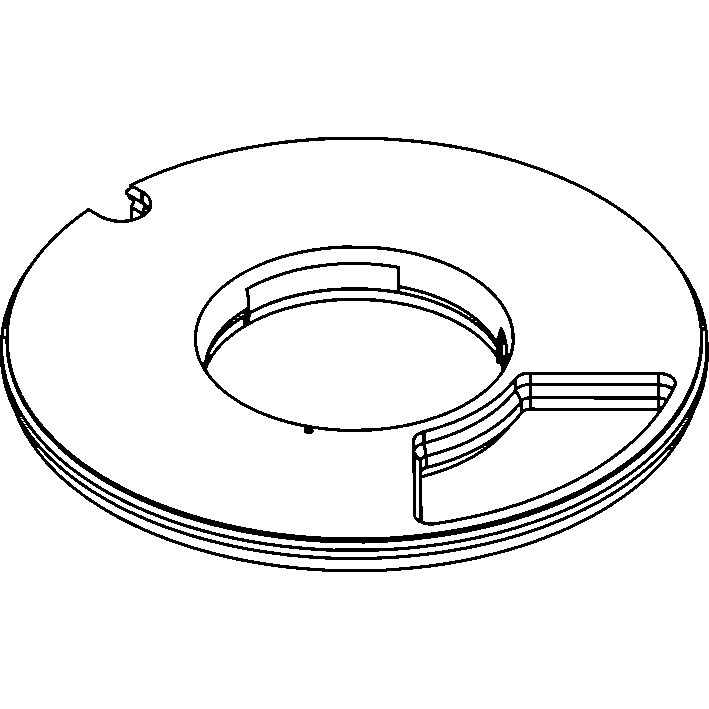
\includegraphics[height=3cm]{images/wireframes/bucket_lid.png}
        \captionof*{figure}{1x Bucket Lid}
    \end{minipage}
    \hfill
    \begin{minipage}{0.3\textwidth}
        \centering
        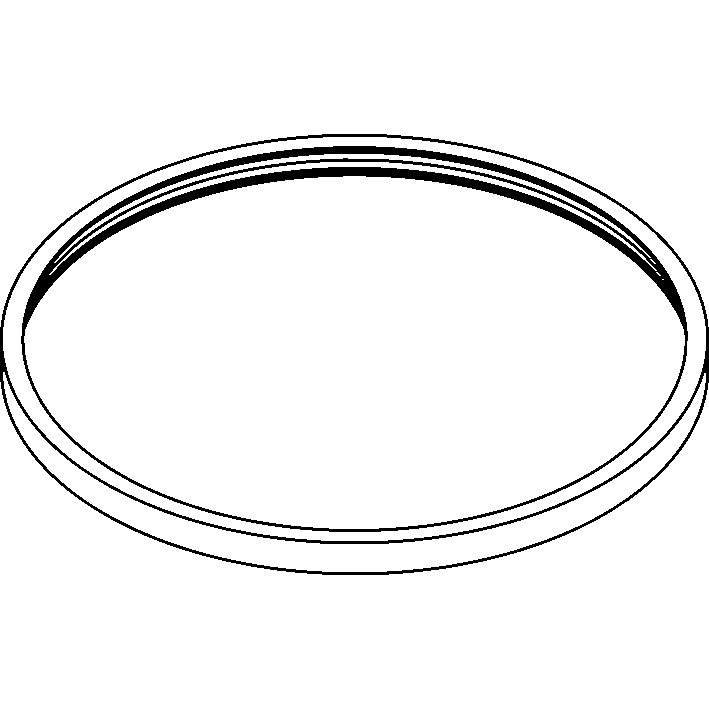
\includegraphics[height=3cm]{images/wireframes/bucket_lid_lockring.png}
        \captionof*{figure}{1x Bucket lid lock-ring}
    \end{minipage}
    \hfill
    \begin{minipage}{0.3\textwidth}
        \centering
        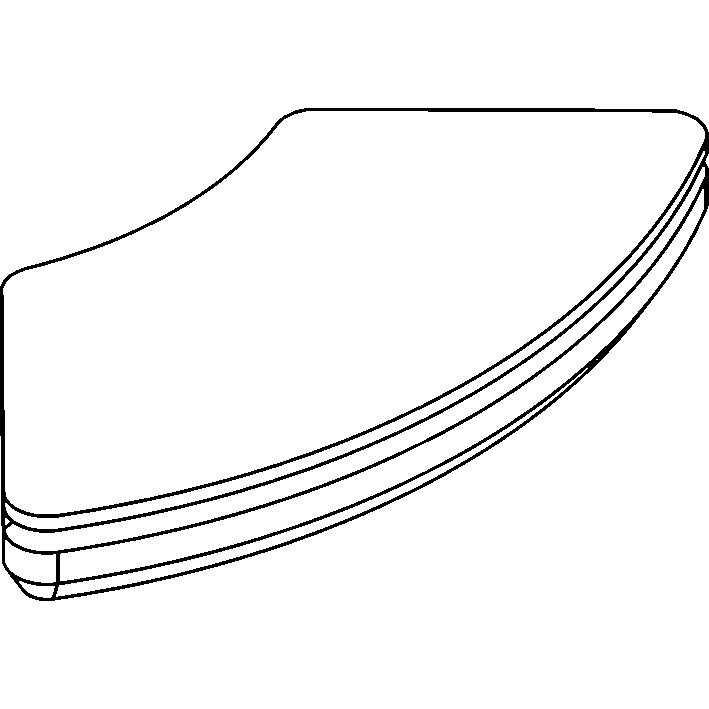
\includegraphics[height=3cm]{images/wireframes/bucket_lid_cap.png}
        \captionof*{figure}{1x Bucket lid cap}
    \end{minipage}

    \vspace{8pt}
    \rule{\textwidth}{0.5pt}
    \vspace{2pt}

    \begin{minipage}{0.3\textwidth}
        \centering
        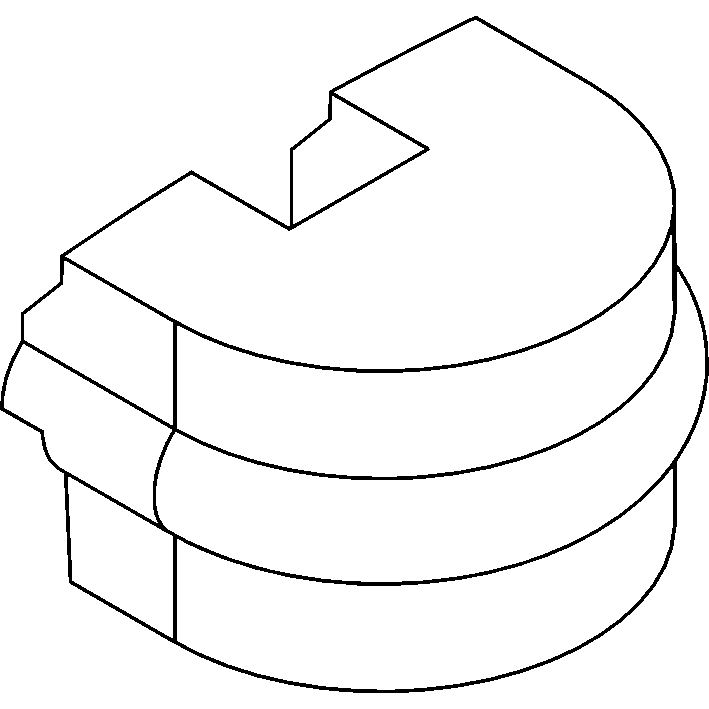
\includegraphics[height=3cm]{images/wireframes/cable_gland_2wire.png}
        \captionof*{figure}{1x Two-wire cable gland}
    \end{minipage}
    \hfill
    \begin{minipage}{0.3\textwidth}
        \centering
        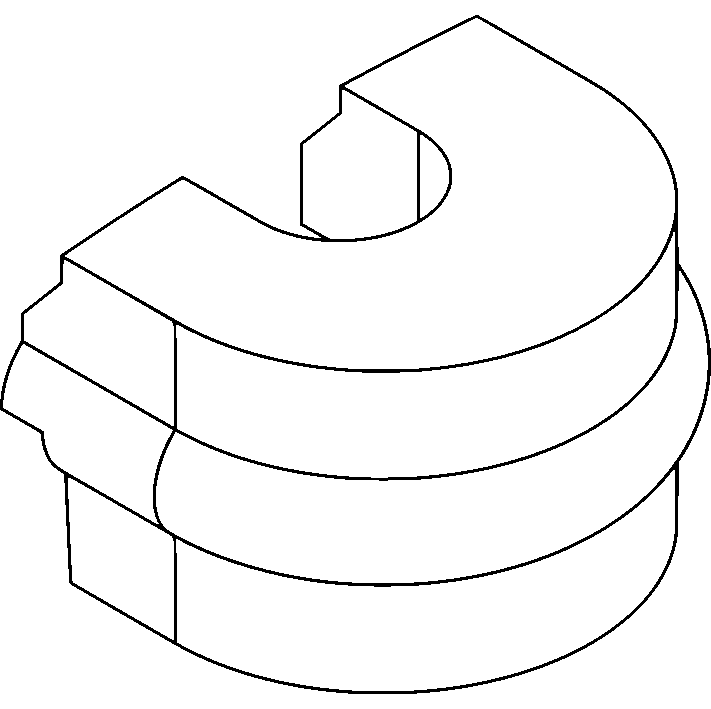
\includegraphics[height=3cm]{images/wireframes/cable_gland_3wire.png}
        \captionof*{figure}{1x Three-wire cable gland}
    \end{minipage}
    \hfill
    \begin{minipage}{0.3\textwidth}
        \centering
        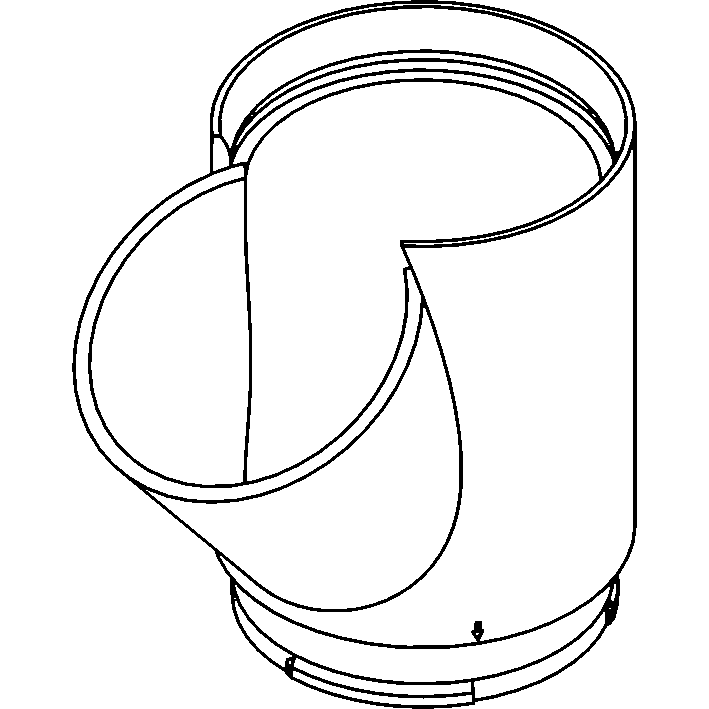
\includegraphics[height=3cm]{images/wireframes/80mm_base_module.png}
        \captionof*{figure}{1x Twist-lock base module}
    \end{minipage}

    \vspace{8pt}
    \rule{\textwidth}{0.5pt}
    \vspace{2pt}

    \begin{minipage}{0.3\textwidth}
        \centering
        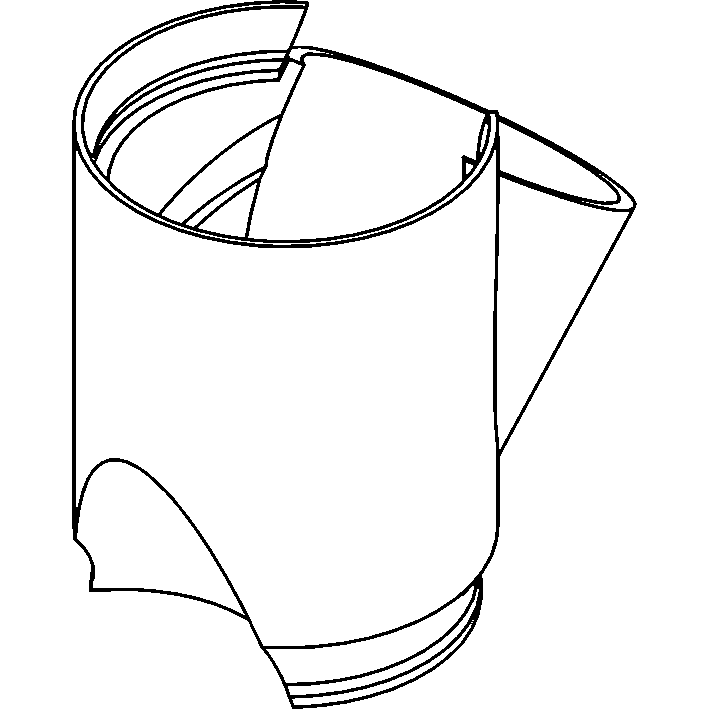
\includegraphics[height=3cm]{images/wireframes/80mm_module.png}
        \captionof*{figure}{4x Snap-fit module}
    \end{minipage}
    \hfill
    \begin{minipage}{0.3\textwidth}
        \centering
        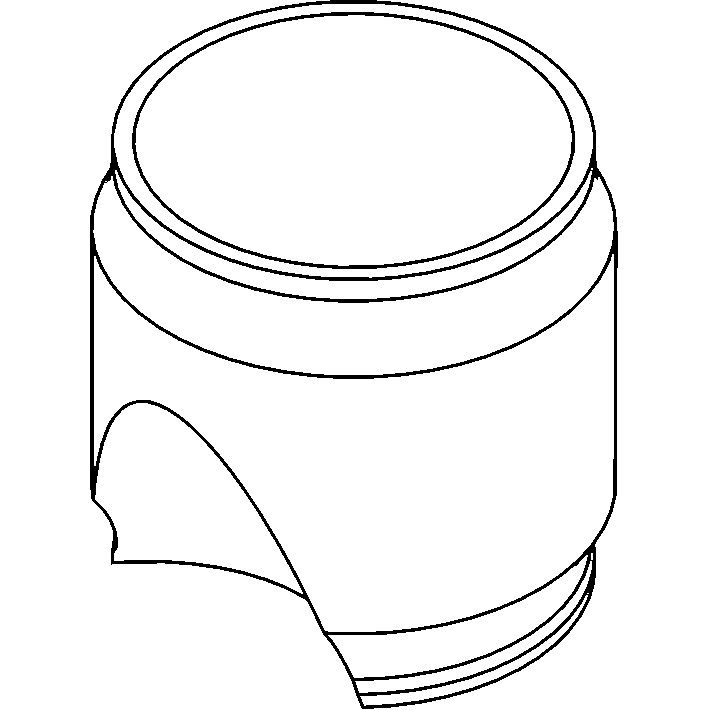
\includegraphics[height=3cm]{images/wireframes/80mm_chimney.png}
        \captionof*{figure}{1x Chimney module}
    \end{minipage}
    \hfill
    \begin{minipage}{0.3\textwidth}
        \centering
        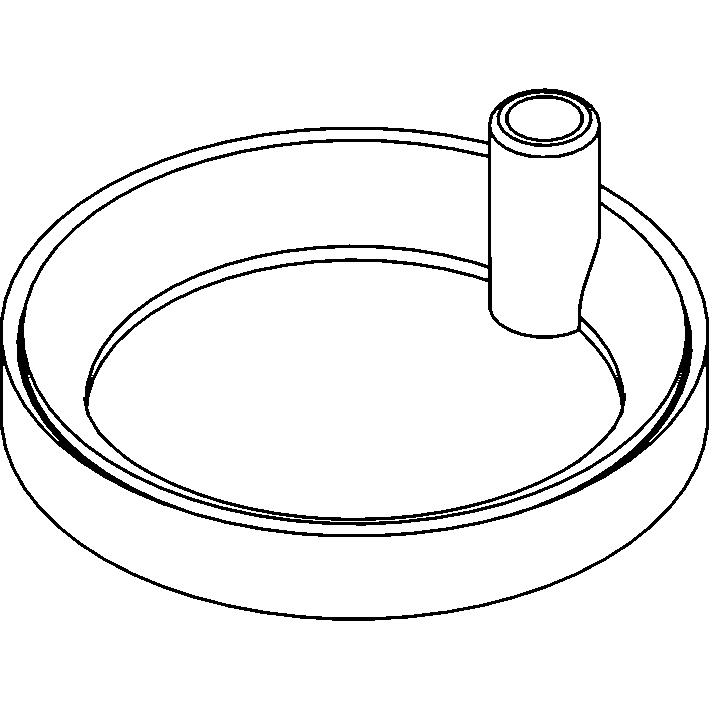
\includegraphics[height=3cm]{images/wireframes/80mm_shower_head.png}
        \captionof*{figure}{1x Shower head}
    \end{minipage}

    % \vspace{8pt}
    % \rule{\textwidth}{0.5pt}
    % \vspace{2pt}

    \begin{minipage}{0.3\textwidth}
        \centering
        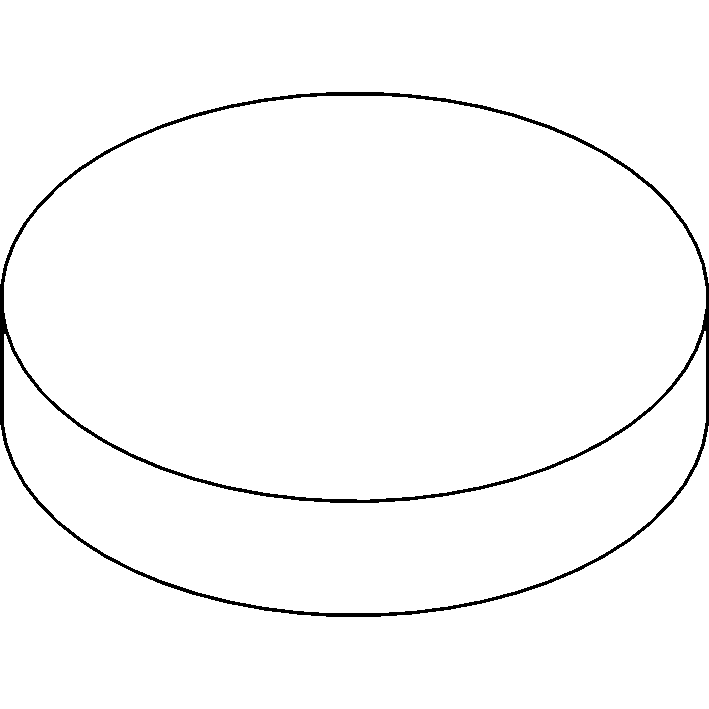
\includegraphics[height=3cm]{images/wireframes/chimney_lid.png}
        \captionof*{figure}{1x Chimney lid}
    \end{minipage}
    \hfill
    \begin{minipage}{0.3\textwidth}
        \centering
        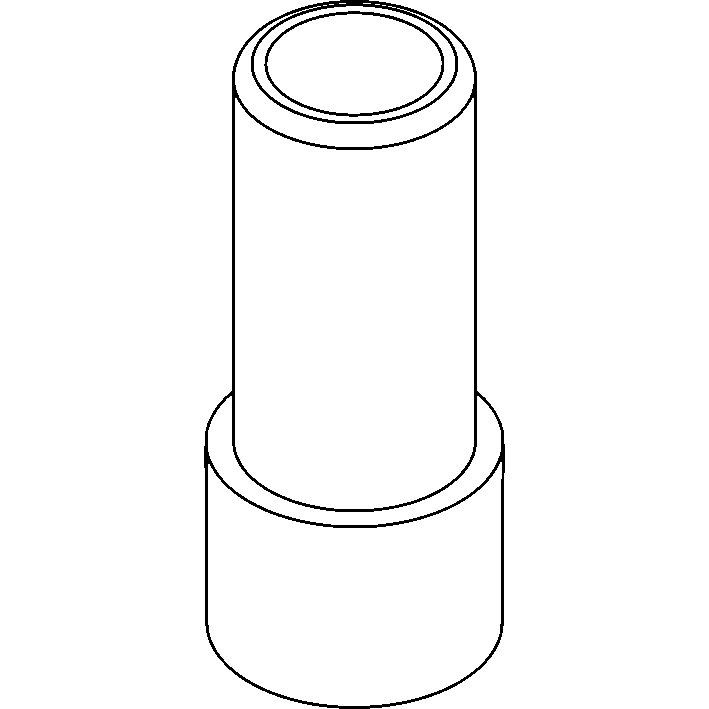
\includegraphics[height=3cm]{images/wireframes/adapter_13mm.png}
        \captionof*{figure}{1x 13mm hose adapter}
    \end{minipage}
    \hfill
    \begin{minipage}{0.3\textwidth}
        \centering
        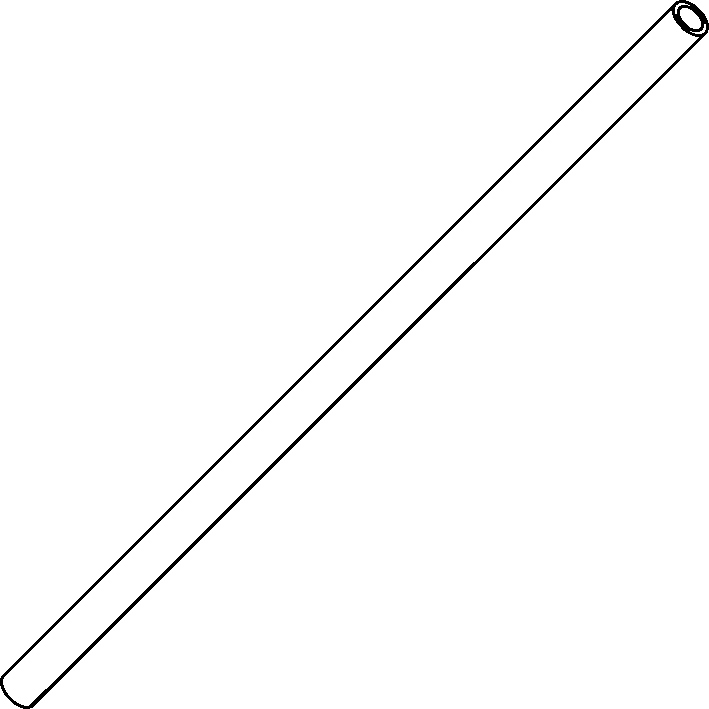
\includegraphics[height=3cm]{images/wireframes/hose_13mm.png}
        \captionof*{figure}{1x 13mm Hose}
    \end{minipage}

    \vspace{8pt}
    \rule{\textwidth}{0.5pt}
    \vspace{2pt}

    \begin{minipage}{0.3\textwidth}
        \centering
        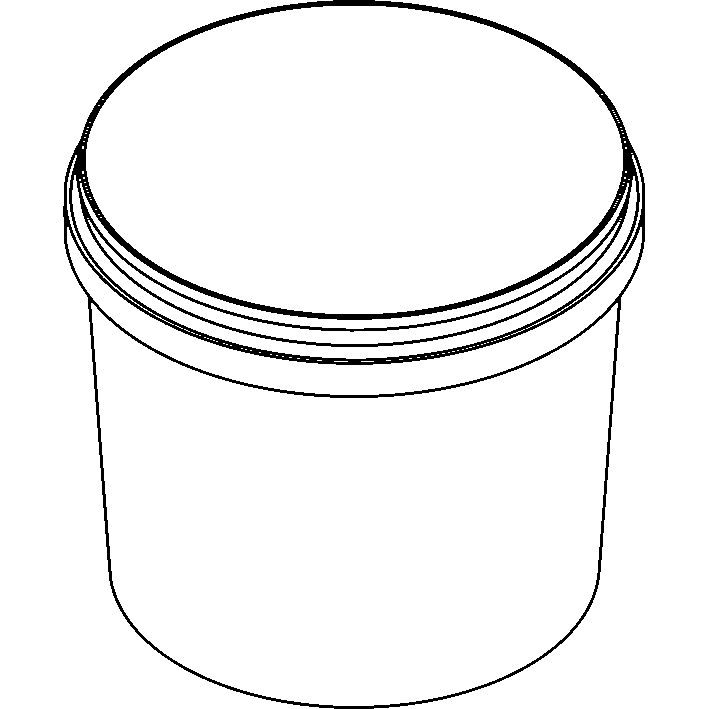
\includegraphics[height=3cm]{images/wireframes/bucket_5l.png}
        \captionof*{figure}{1x 5L Bucket}
    \end{minipage}
\end{center}

\clearpage

\setlength{\intextsep}{15.0pt plus 0.0pt minus 0.0pt}
\setlength{\floatsep}{0.0pt plus 0.0pt minus 0.0pt}
\setlength{\textfloatsep}{15.0pt plus 0.0pt minus 0.0pt}
\setlength{\belowcaptionskip}{-20.0pt}

\subsection{Assembly}

\begin{enumerate}

\item Align the arrow at the base of the \textbf{twist-lock base module} with the arrow on the top of the \textbf{bucket lid}. Carefully insert the base of the module into the hole in the center of the bucket lid when the arrows are aligned.

\item Once the \textbf{twist-lock base module} is inserted into the \textbf{bucket lid}, twist the module clockwise until you feel it stop. \textbf{Do not twist past this point.}

\begin{figure}[h]
    \centering
    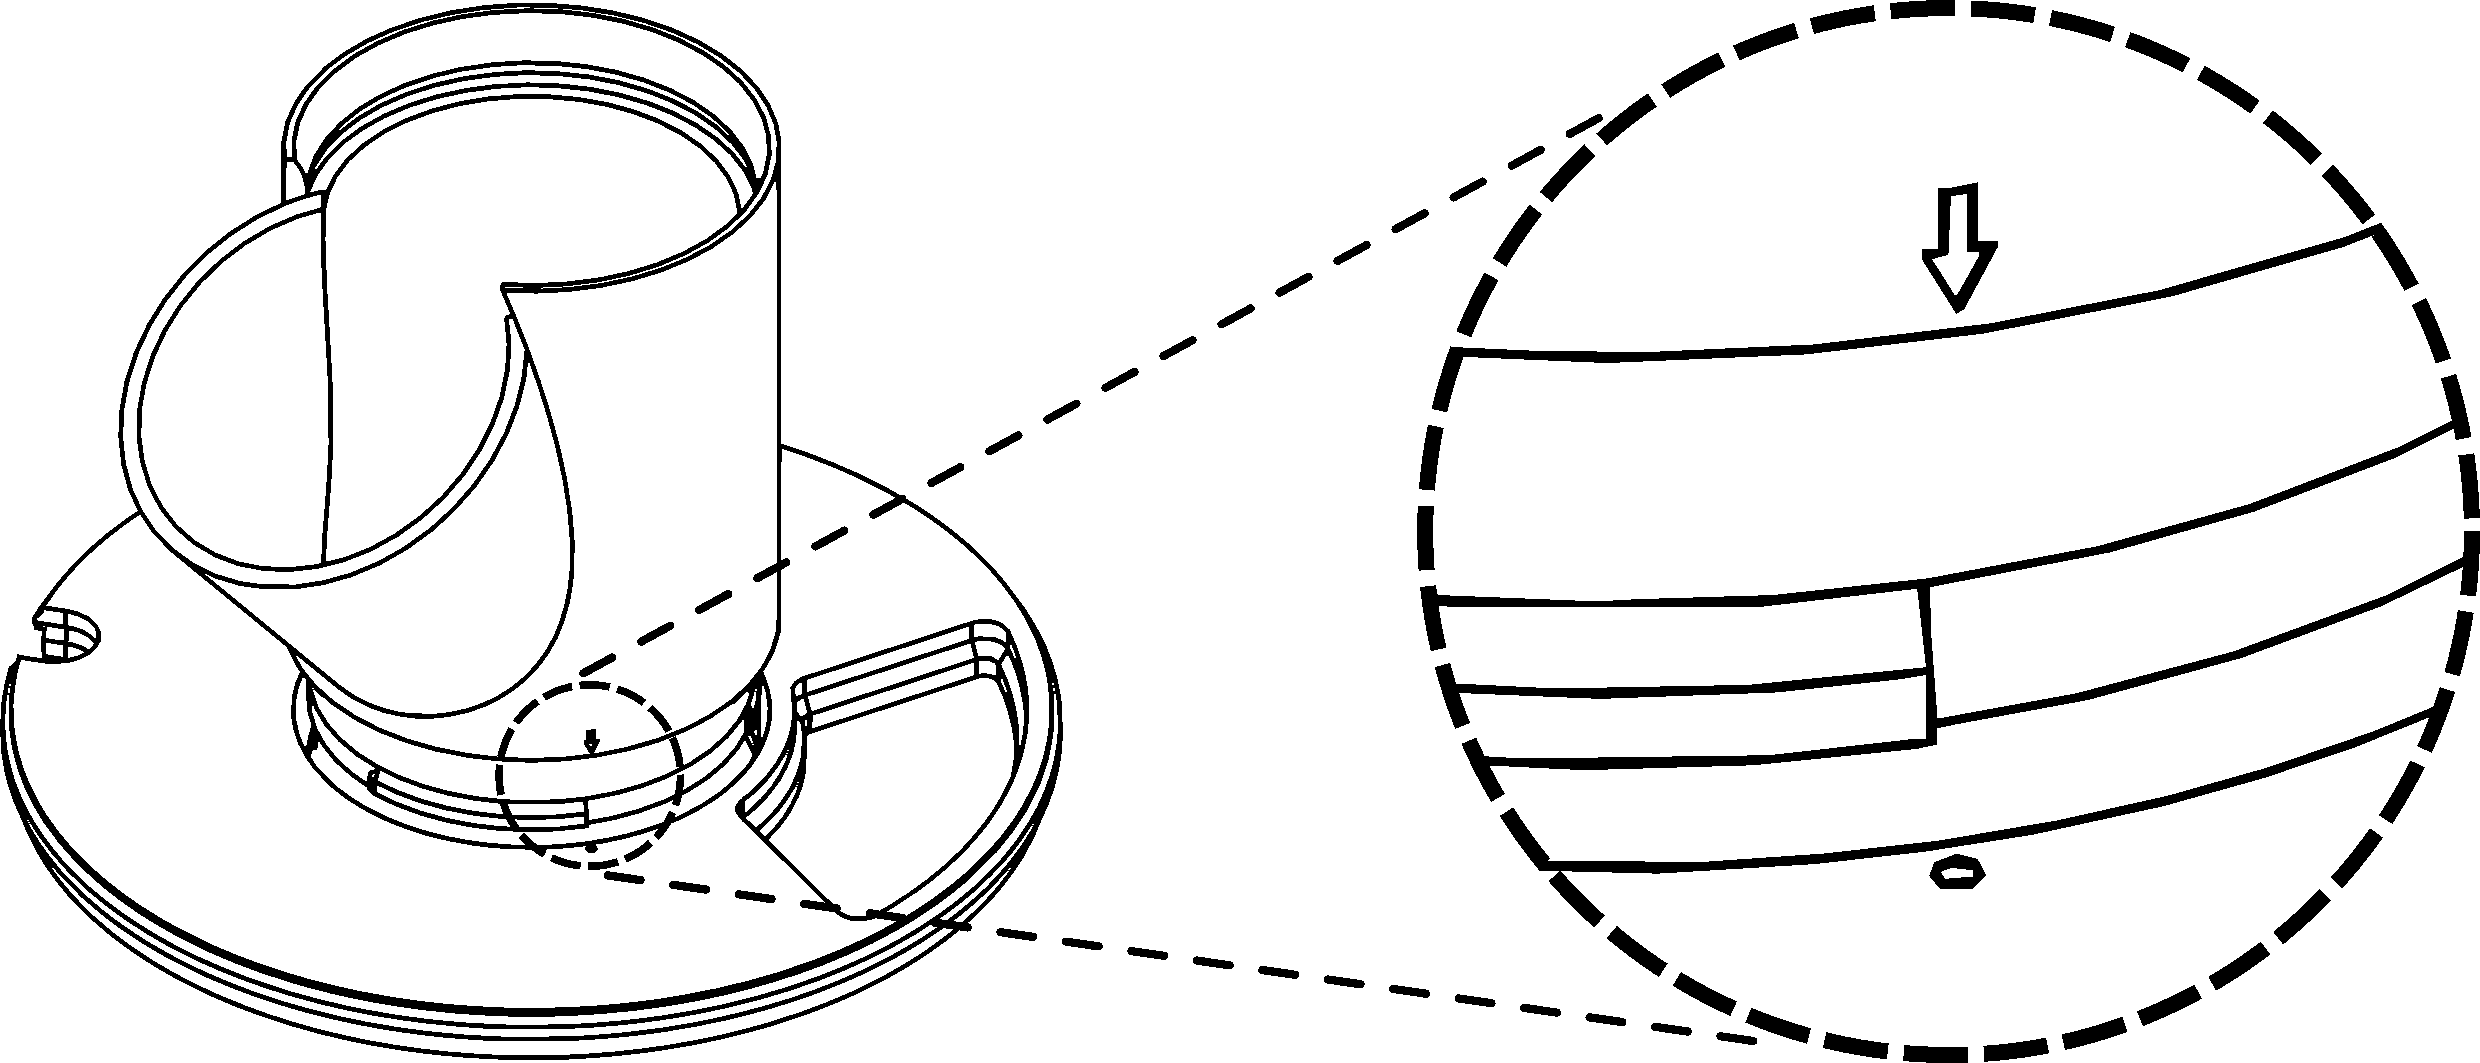
\includegraphics[width=0.8\textwidth]{images/80mm/80mm_assembly_1.png}
    \caption*{}
    \label{fig:80mm-one}
\end{figure}
\begin{figure}[h!]
    \centering
    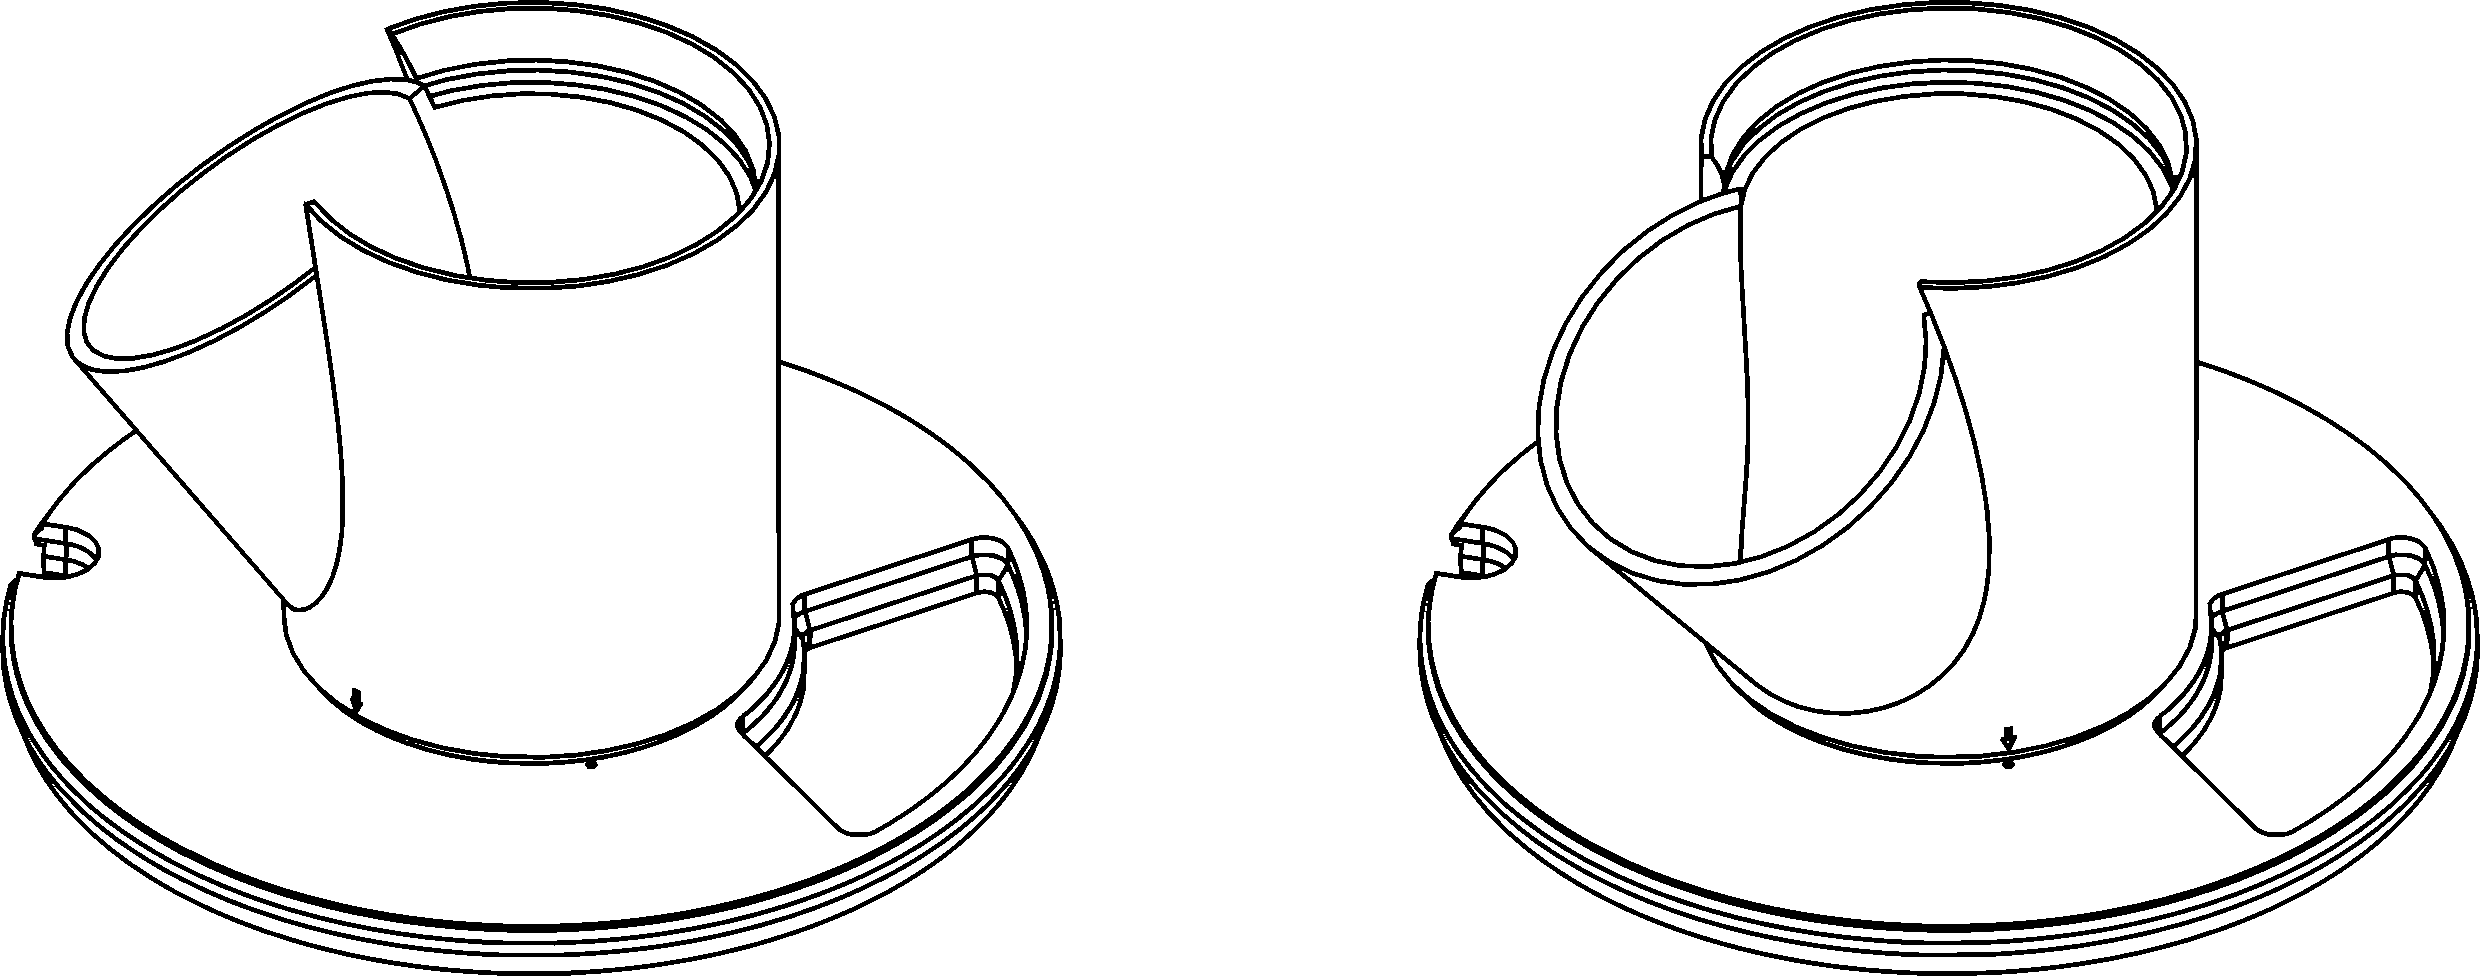
\includegraphics[width=0.8\textwidth]{images/80mm/80mm_assembly_2.png}
    \caption*{}
    \label{fig:80mm-two}
\end{figure}

\item Align the bottom of a \textbf{snap-fit module} with the top of the \textbf{twist-lock base module} so that the net pot receptacles of each module are facing 180 degrees away from one another.

\item With the pot receptacle of the lower module facing toward you, first push the \textbf{rear} of the upper module down into the snap-fit receiver of the lower module.

\item With the rear of the upper module seated in the snap-fit receiver of the lower module, carefully push down the \textbf{fore} of the upper module into the snap-fit receiver of the lower module. The foot of the upper module should seat fully into the snap-fit receiver of the lower module.

\begin{figure}[h]
    \centering
    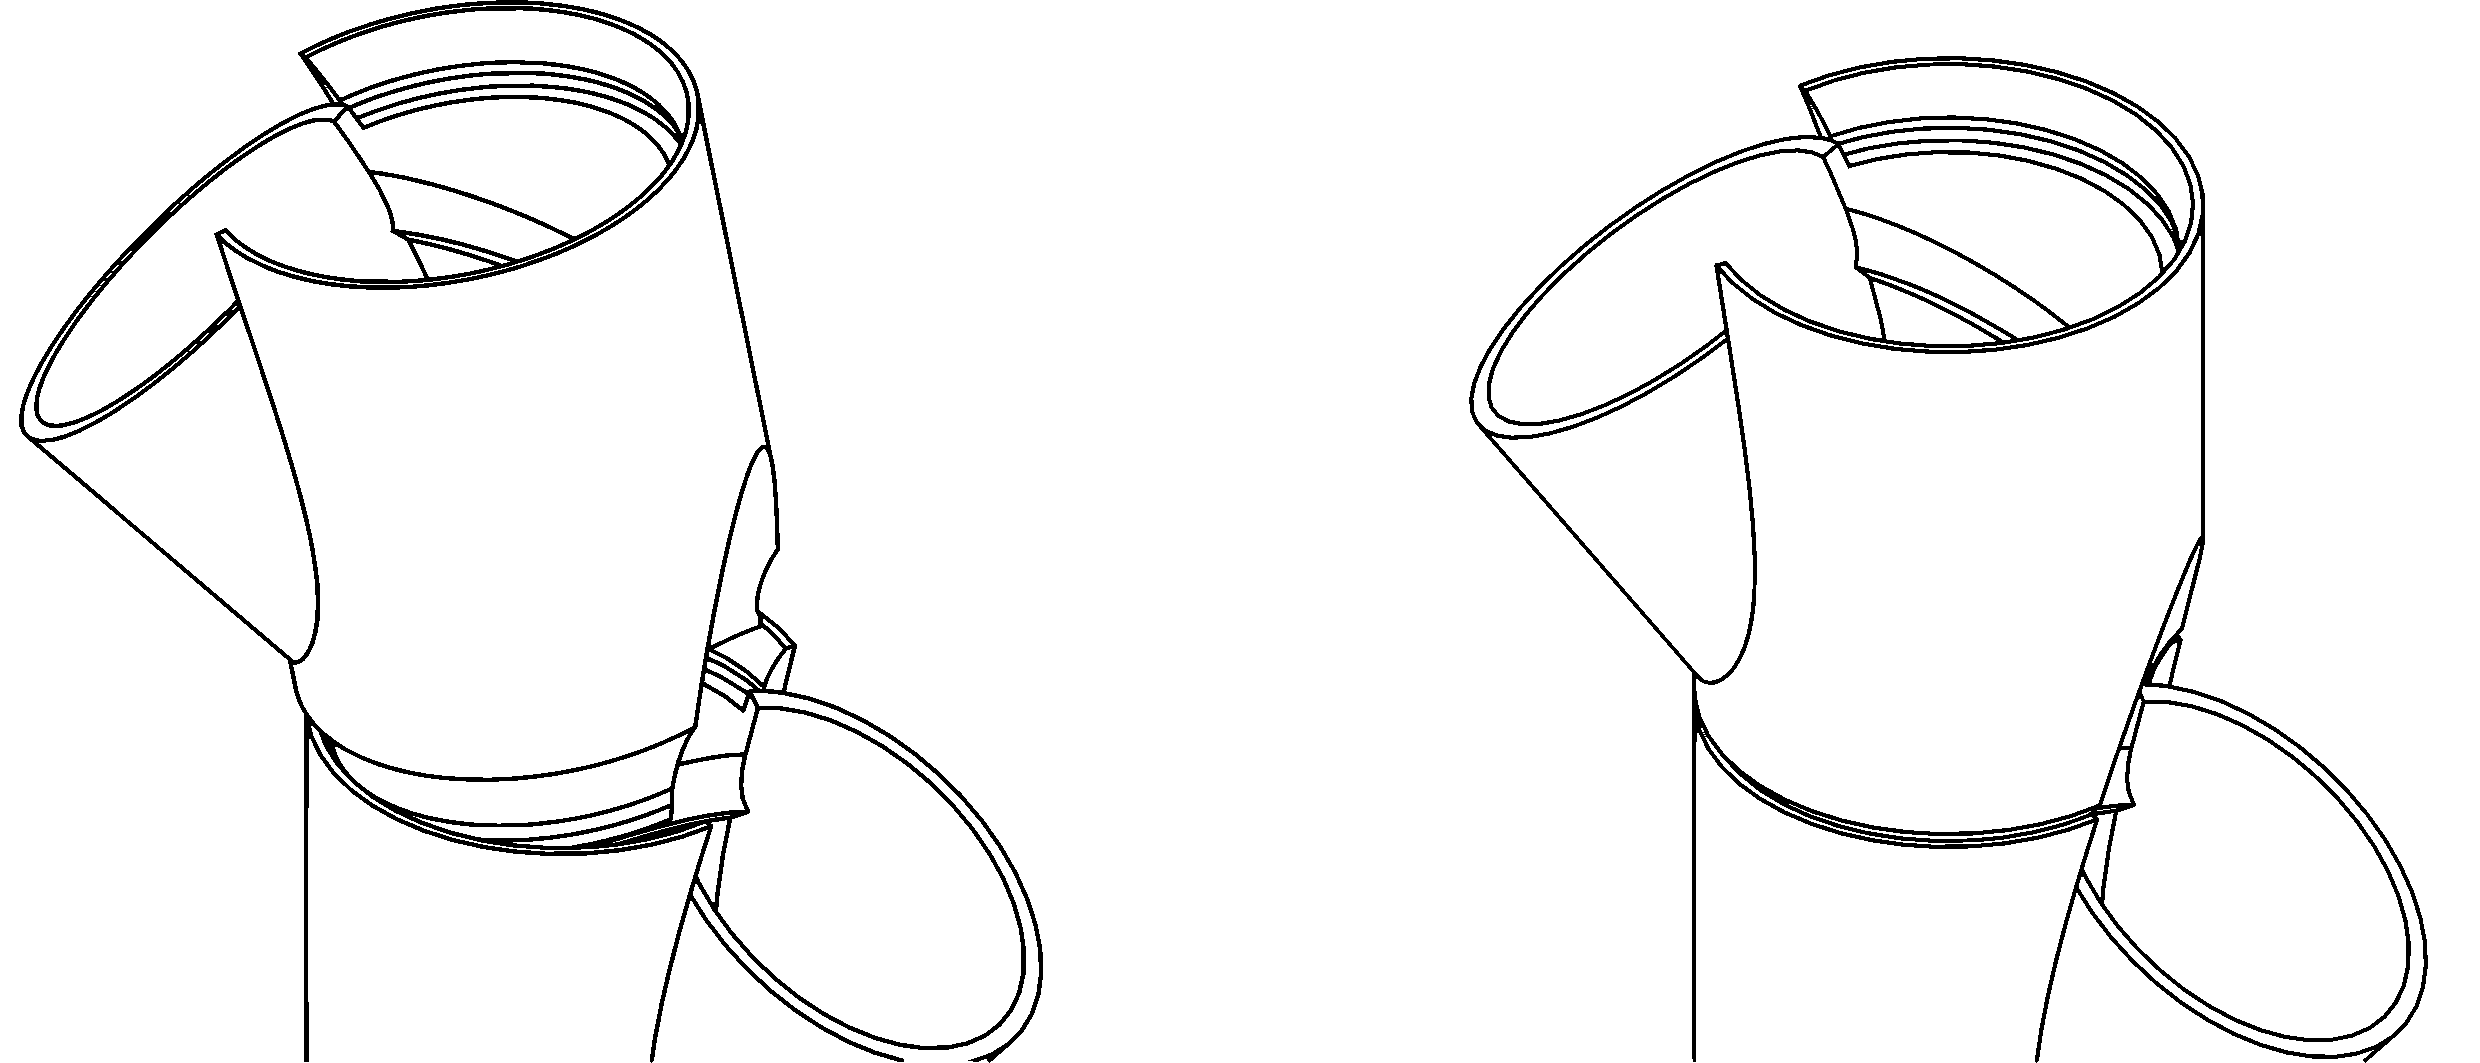
\includegraphics[width=0.8\textwidth]{images/80mm/80mm_assembly_3.png}
    \caption*{}
    \label{fig:80mm-three}
\end{figure}
\begin{figure}[h!]
    \centering
    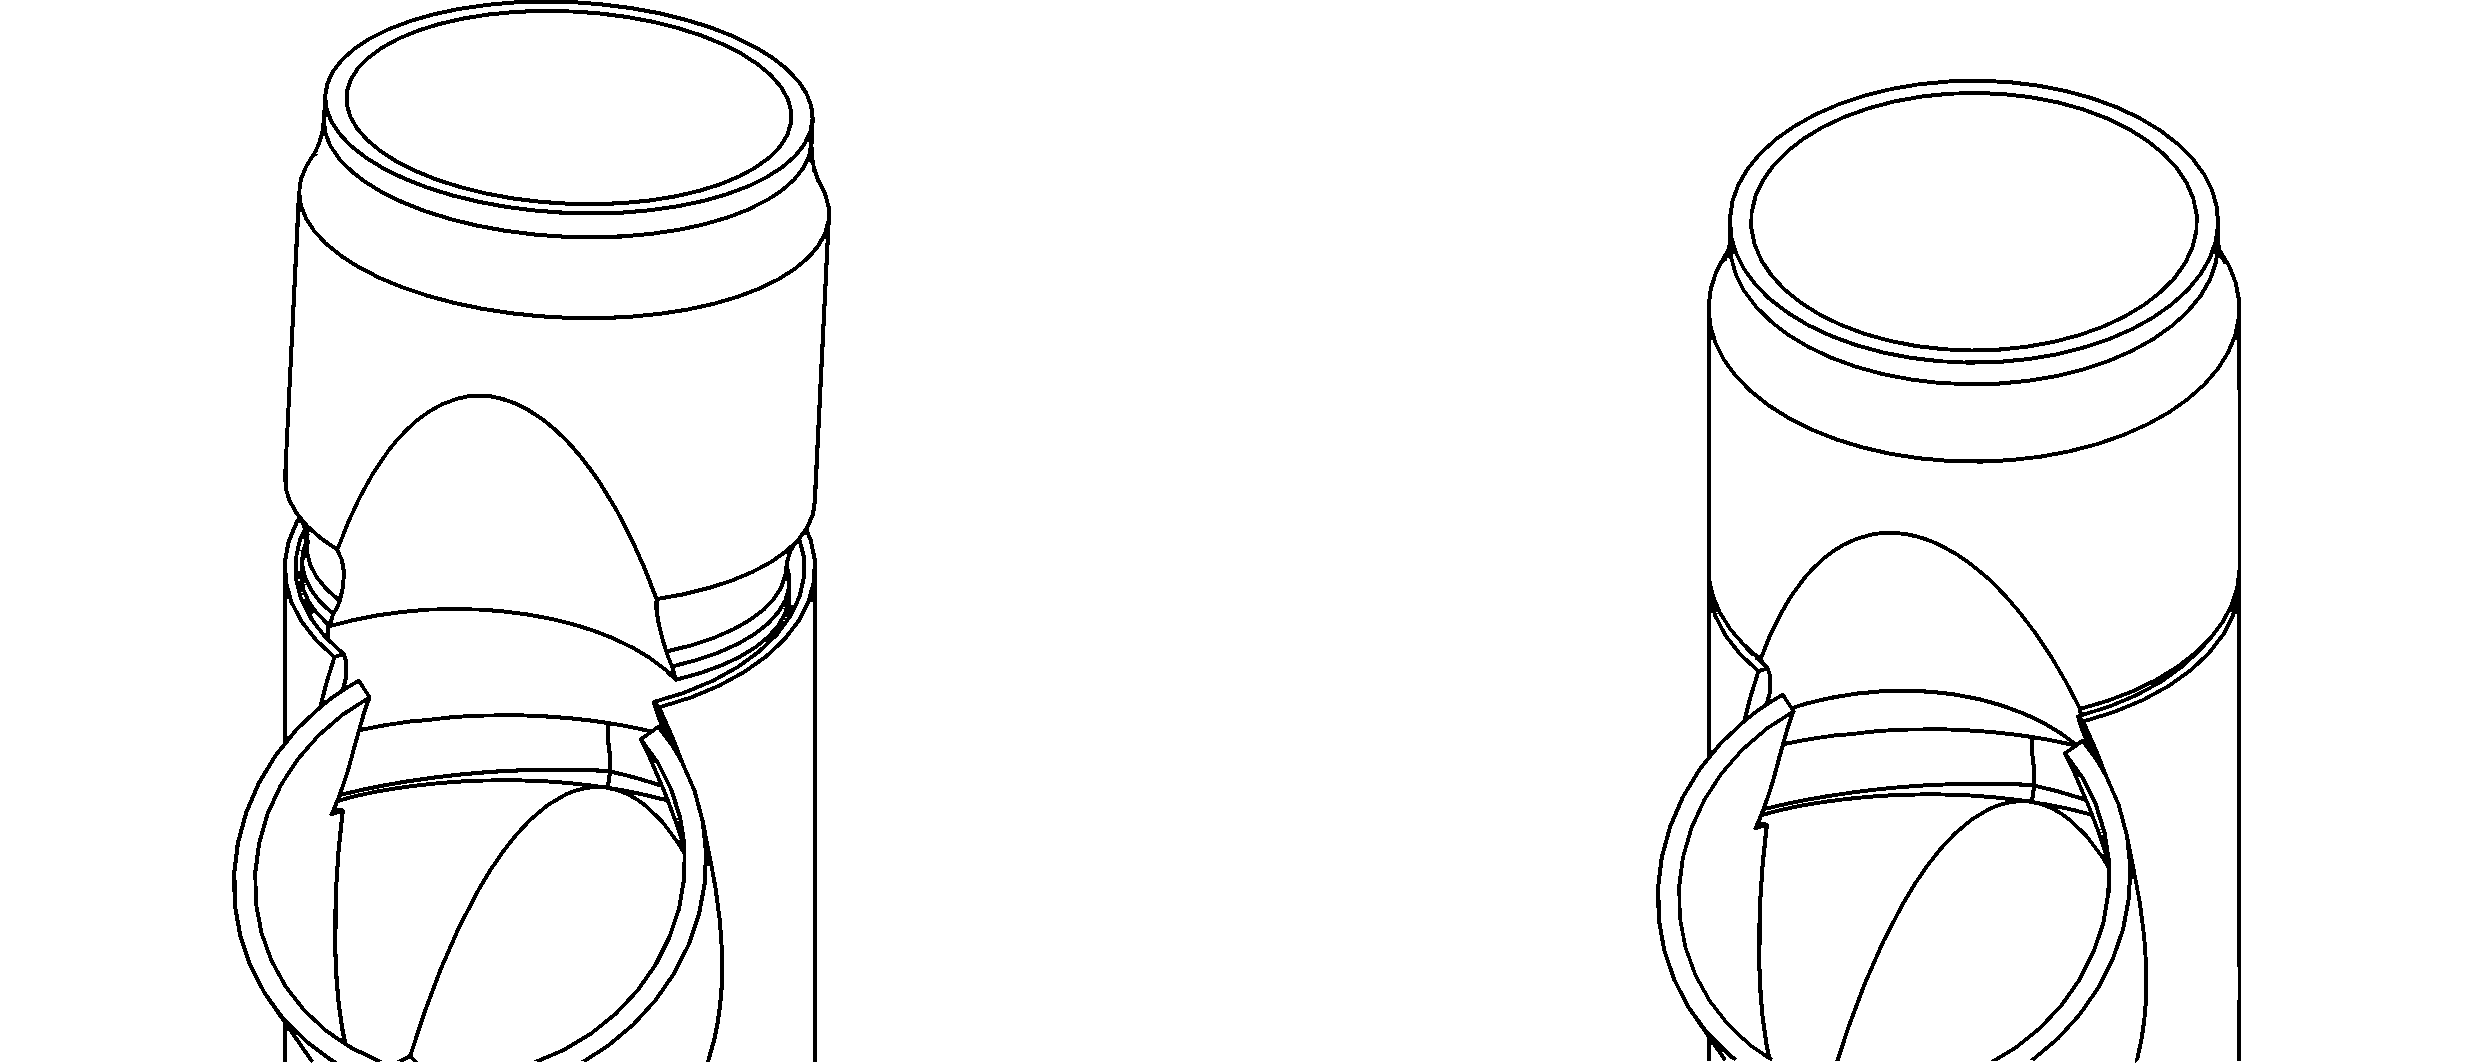
\includegraphics[width=0.8\textwidth]{images/80mm/80mm_assembly_4.png}
    \caption*{}
    \label{fig:80mm-four}
\end{figure}

\item Repeat steps 3 through 5 with the remaining planter modules.

\item Using the same method, insert the \textbf{chimney module} into the snap-fit receiver of the topmost planter module.

\item Insert the water inlet of the \textbf{shower head} into one end of the \textbf{13mm hose}.

\begin{figure}[h!]
    \centering
    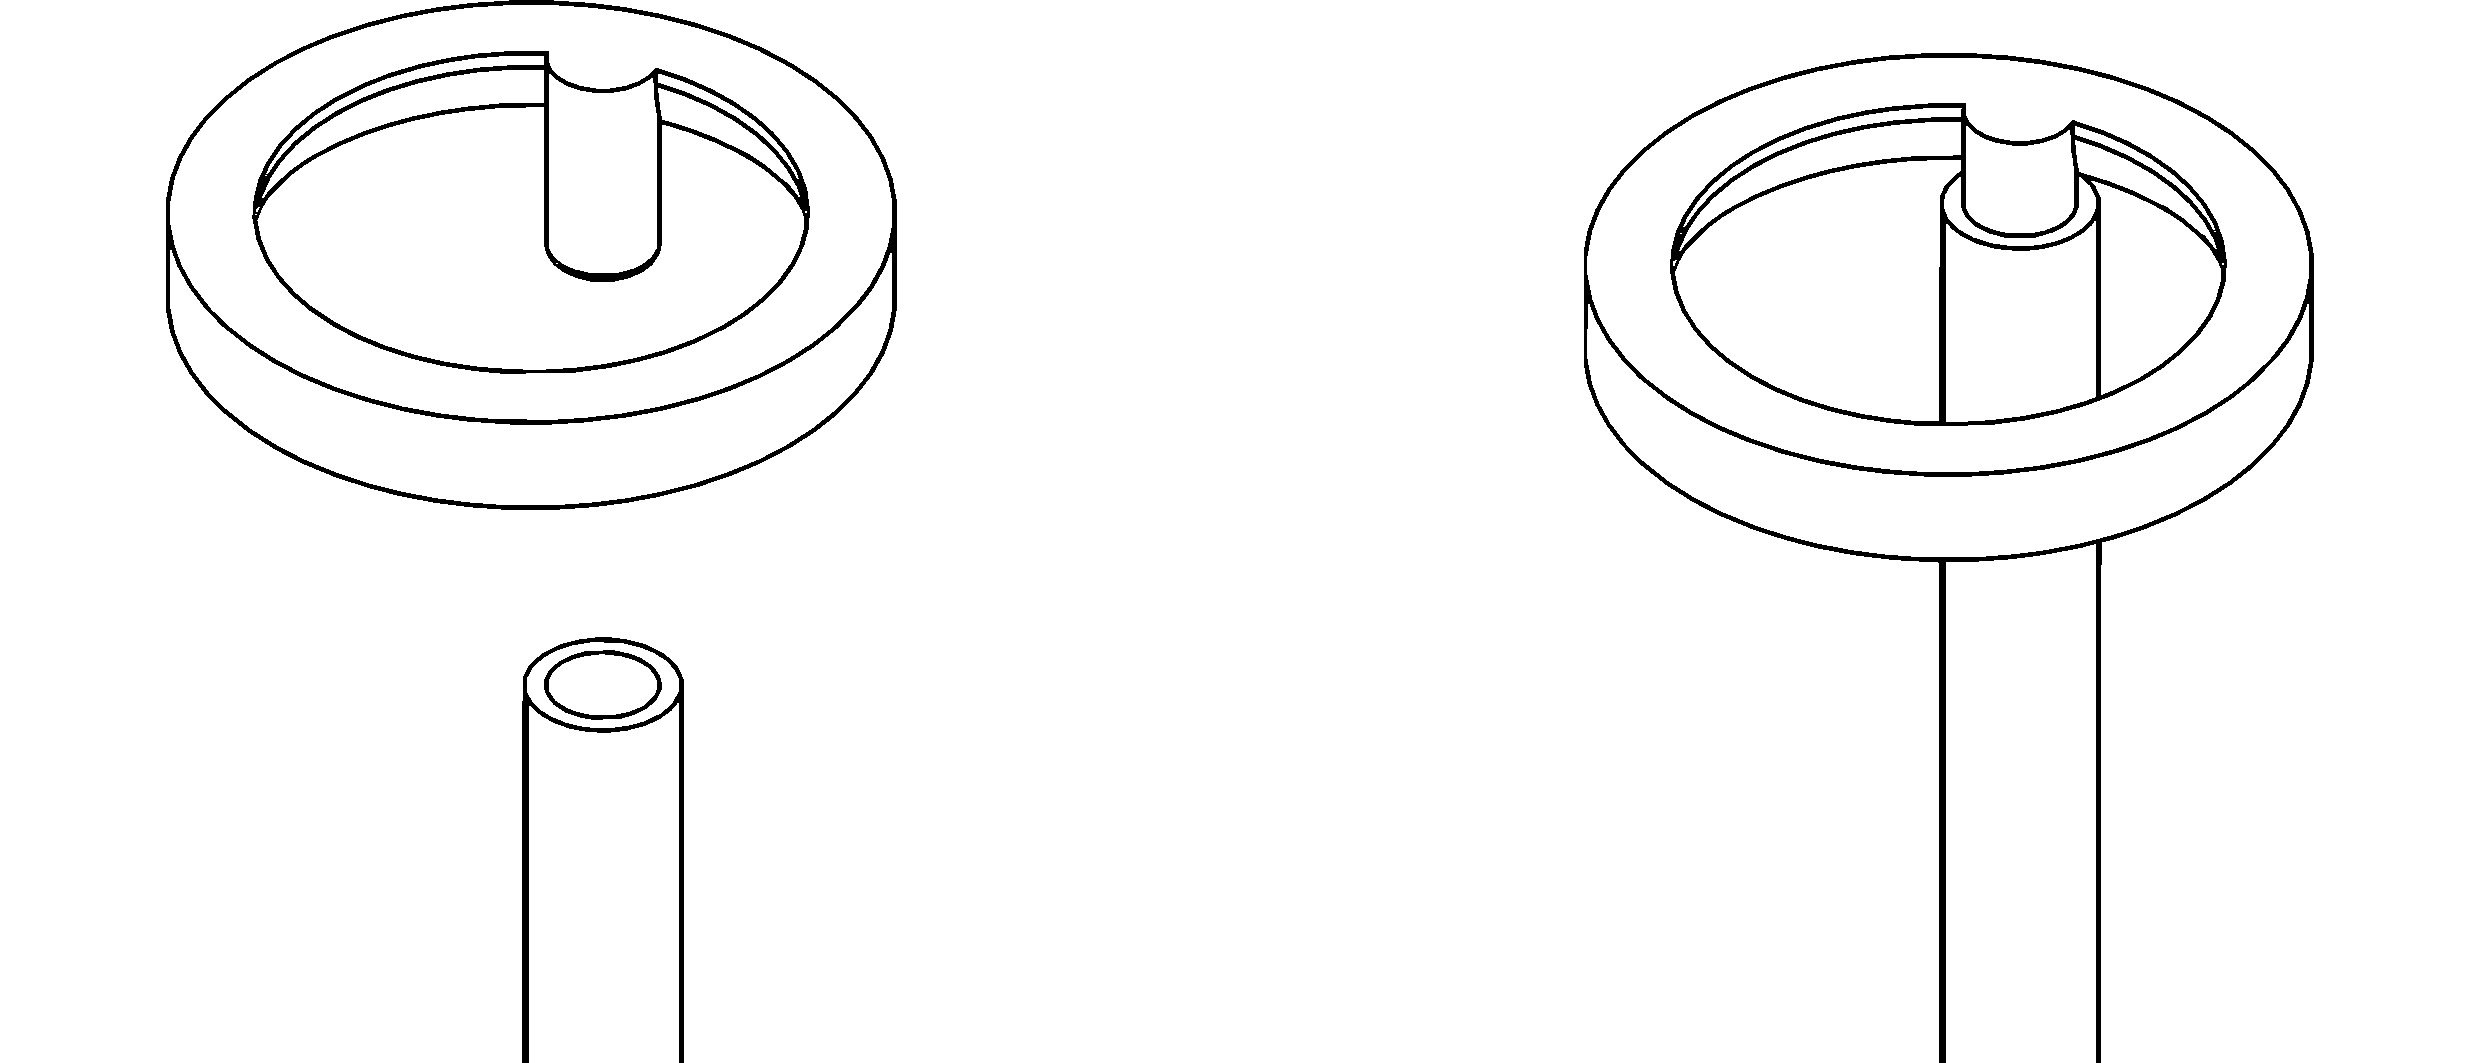
\includegraphics[width=0.8\textwidth]{images/80mm/80mm_assembly_5.png}
    \caption*{}
    \label{fig:80mm-five}
\end{figure}
\begin{figure}[h!]
    \centering
    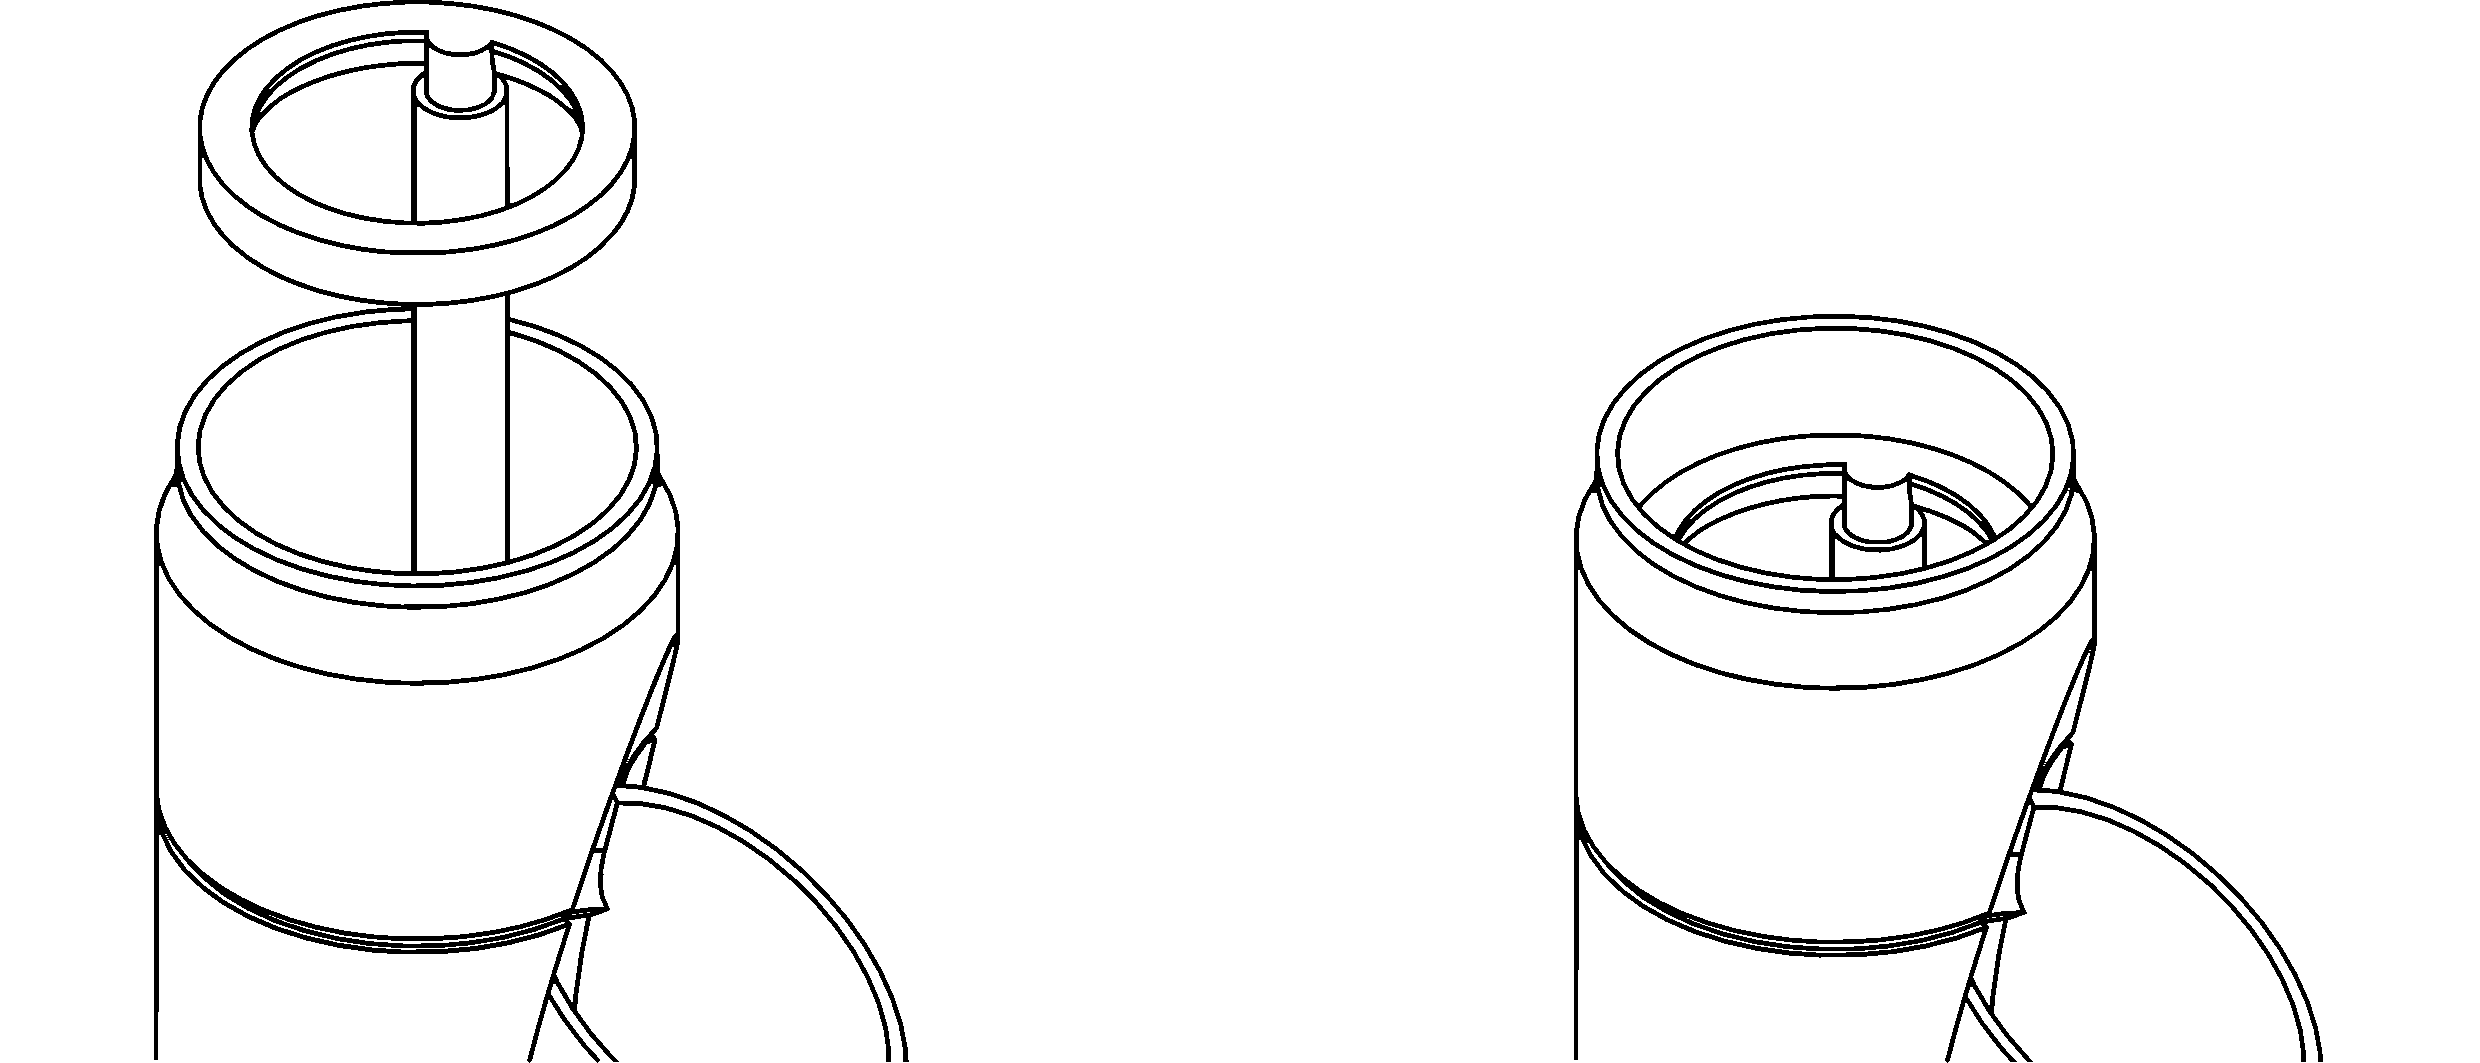
\includegraphics[width=0.8\textwidth]{images/80mm/80mm_assembly_6.png}
    \caption*{}
    \label{fig:80mm-six}
\end{figure}

\item Insert the opposite end of the \textbf{13mm hose} into the tower through the top of the \textbf{chimney module}, then insert the \textbf{shower head} into the top of the chimney module and push it down as far as it will go. Do not force the shower head further into the chimney module than it will go. The shower head is designed to fit snugly into the chimney module to aid the laminar flow of water over the inner wall of the tower, so \textbf{be careful not to angle the shower head as you insert it.}

\item If needed, twist the shower head so that the hose descends the tower adjacent to the net pot receptacles.

\item Insert the appropriate \textbf{bucket lid cable gland} for your chosen pump's power cord into the cable gland receiver of the \textbf{bucket lid}. Be careful to ensure that the cable gland is oriented correctly, or the bucket lid won't sit properly on the bucket.

\begin{figure}[h!]
    \centering
    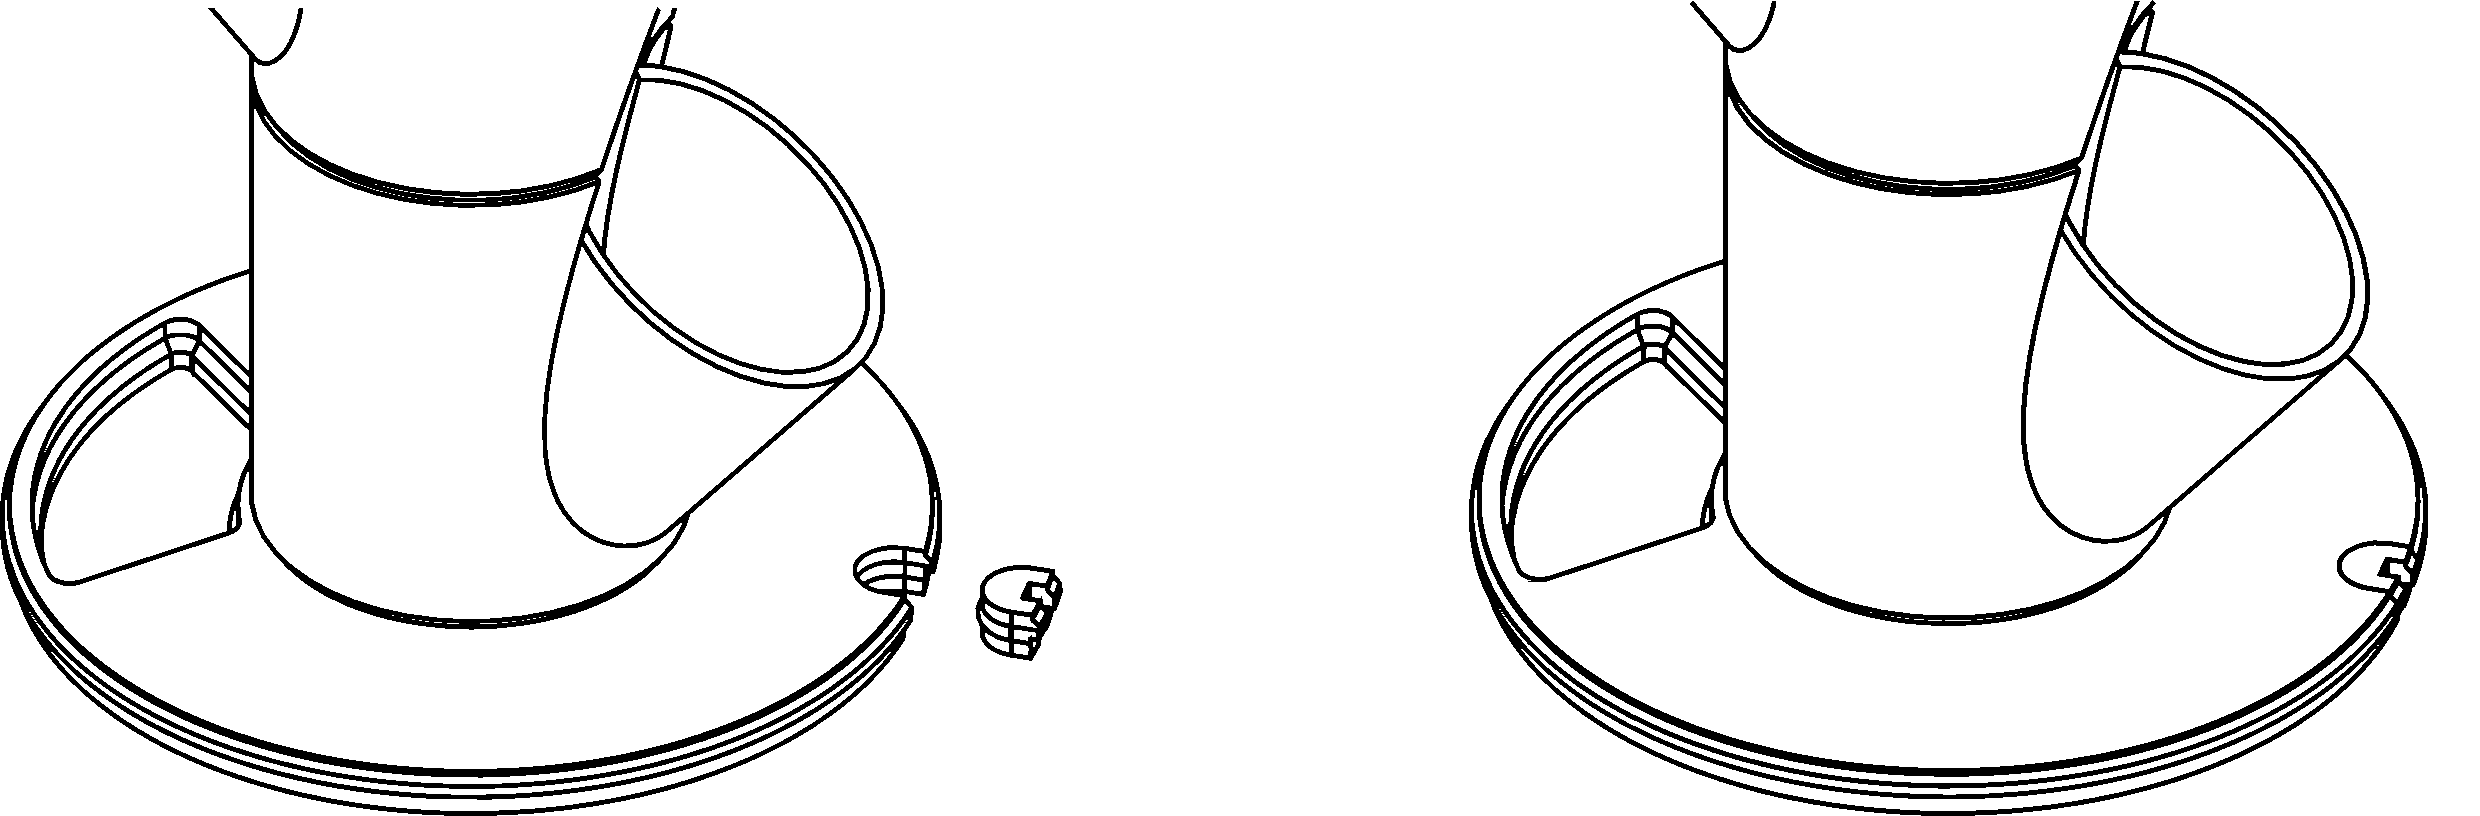
\includegraphics[width=0.8\textwidth]{images/80mm/80mm_assembly_7.png}
    \caption*{}
    \label{fig:80mm-seven}
\end{figure}

\item Place your \textbf{submersible pump} in the \textbf{5L bucket}.

\item If using an Aqua One 103 pump or other Aqua One pump with the same outlet, insert the 13mm end of the \textbf{13mm hose adapter} into the free end of the 13mm hose. If using a different pump, appropriate adapters will need to be provided by the user.

\item While holding the tower so that the bucket lid hovers just above the lip of the bucket, connect the free end of the 13mm hose to the outlet of the submersible pump. You may need to adjust the position of the pump in the bucket to ensure that the pump outlet aligns with the hose.

\item Lower the bucket lid onto the lip of the bucket, ensuring that the power cord of the pump is routed through the bucket lid cable gland. As the bucket lid is lowered, gently pull the shower head upward inside the chimney so that the hose is straightened but not taut.

\begin{figure}[h]
    \centering
    
\includegraphics[width=0.8\textwidth]{images/80mm/80mm_assembly_8.png}
    \caption*{}
    \label{fig:80mm-eight}
\end{figure}

\item Lower the \textbf{bucket lid lock-ring}, with its flat side facing upward, down over the top of the tower. Align the lock-ring with the edge of the bucket lid, then carefully push the lock-ring down into place around the bucket-lid. It may be easiest to work from one point on the lock-ring and around to the other side in both directions simultaneously with both thumbs.

\item Insert the \textbf{bucket lid cap}, with its flat side facing upward, into the cap opening in the bucket lid.

\begin{figure}[h]
    \centering
    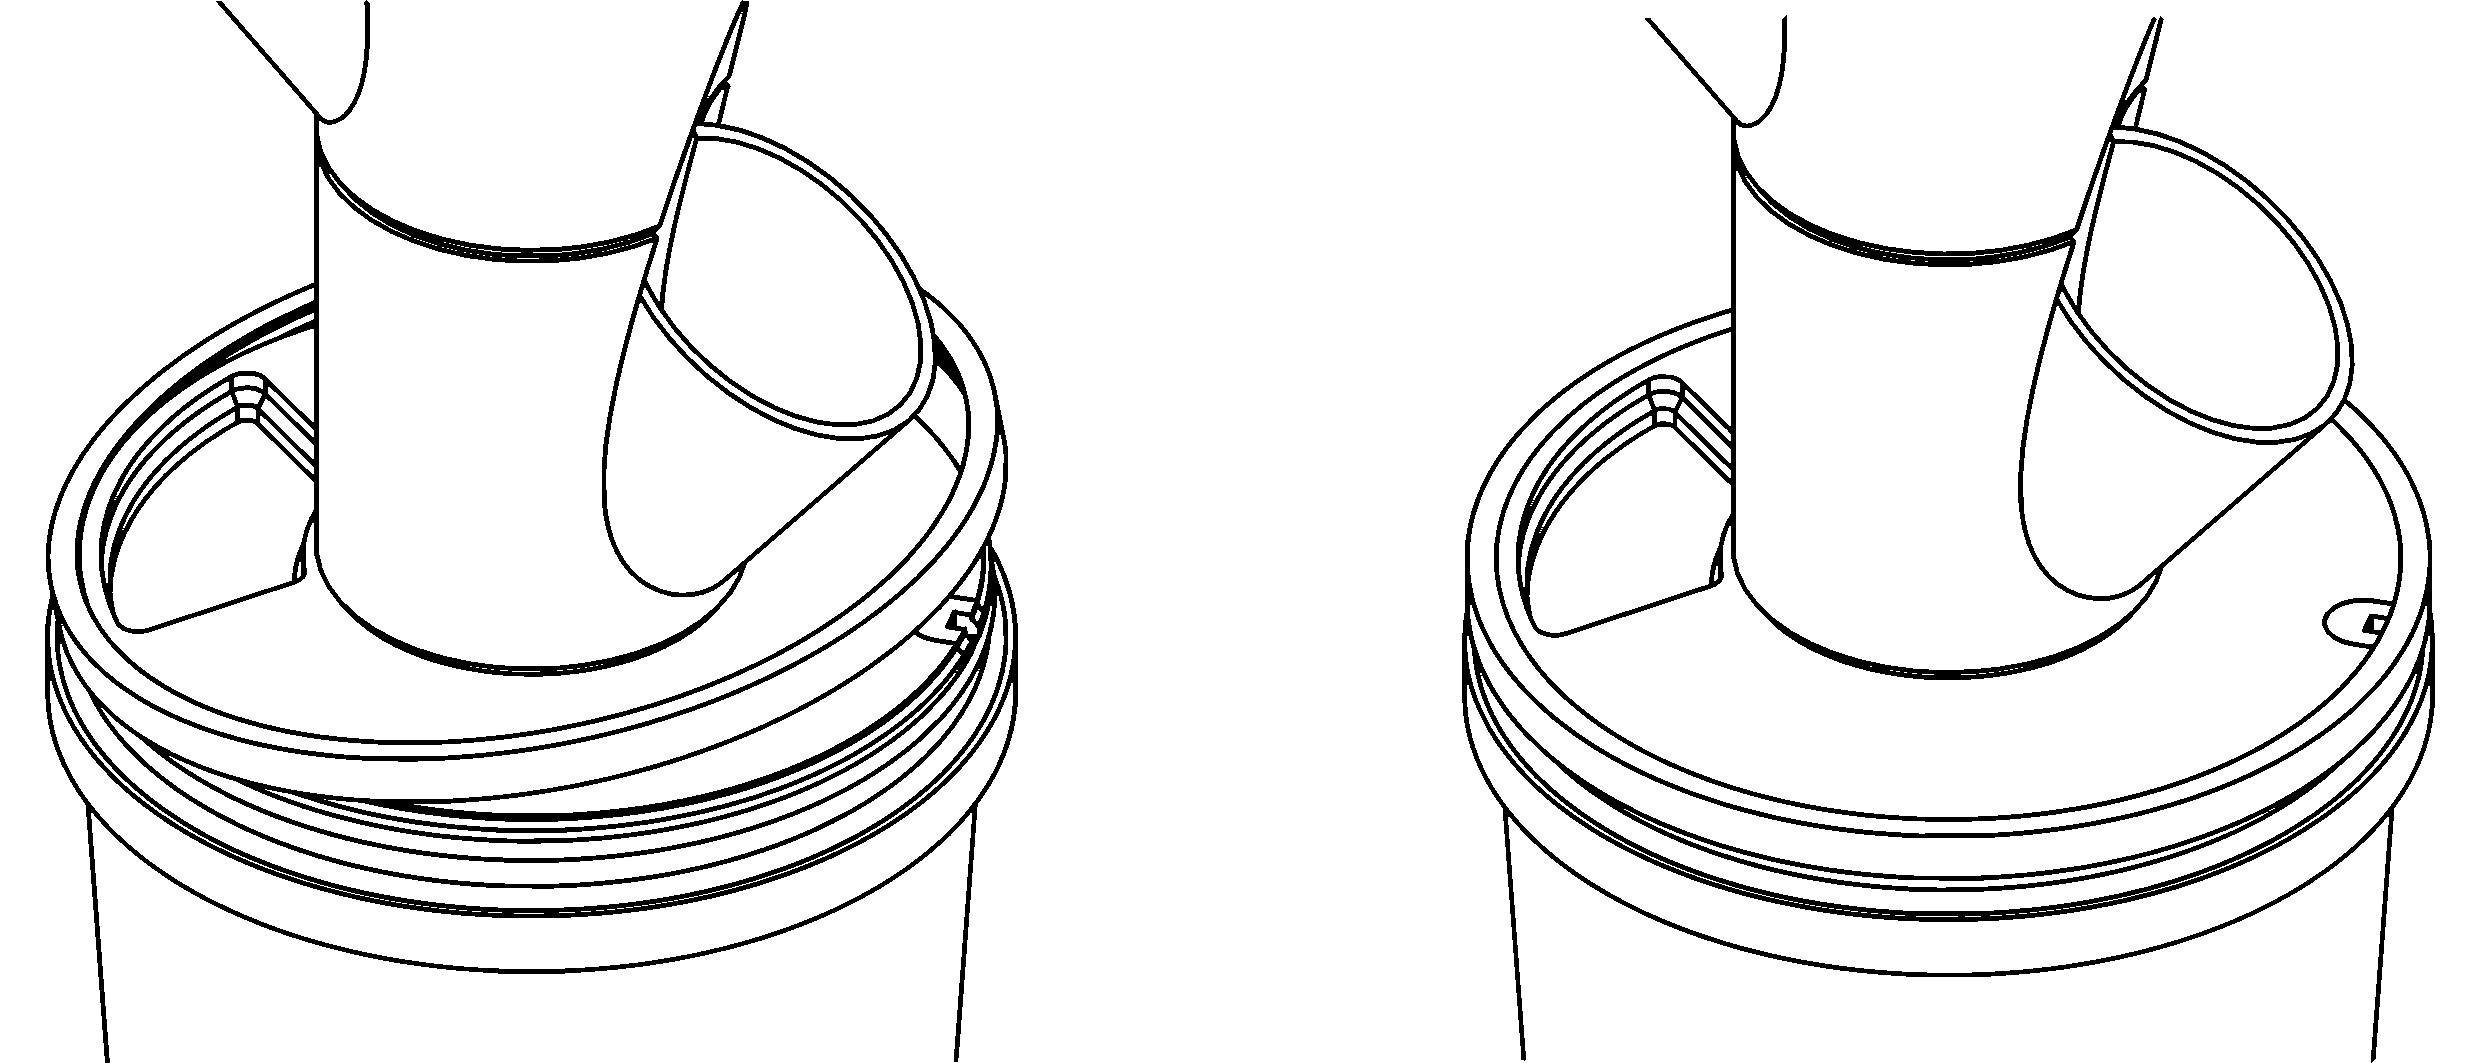
\includegraphics[width=0.8\textwidth]{images/80mm/80mm_assembly_9.png}
    \caption*{}
    \label{fig:80mm-nine}
\end{figure}

\item Place the \textbf{chimney lid}, with its flat side facing upward, on top of the tower chimney.

\begin{figure}[h]
    \centering
    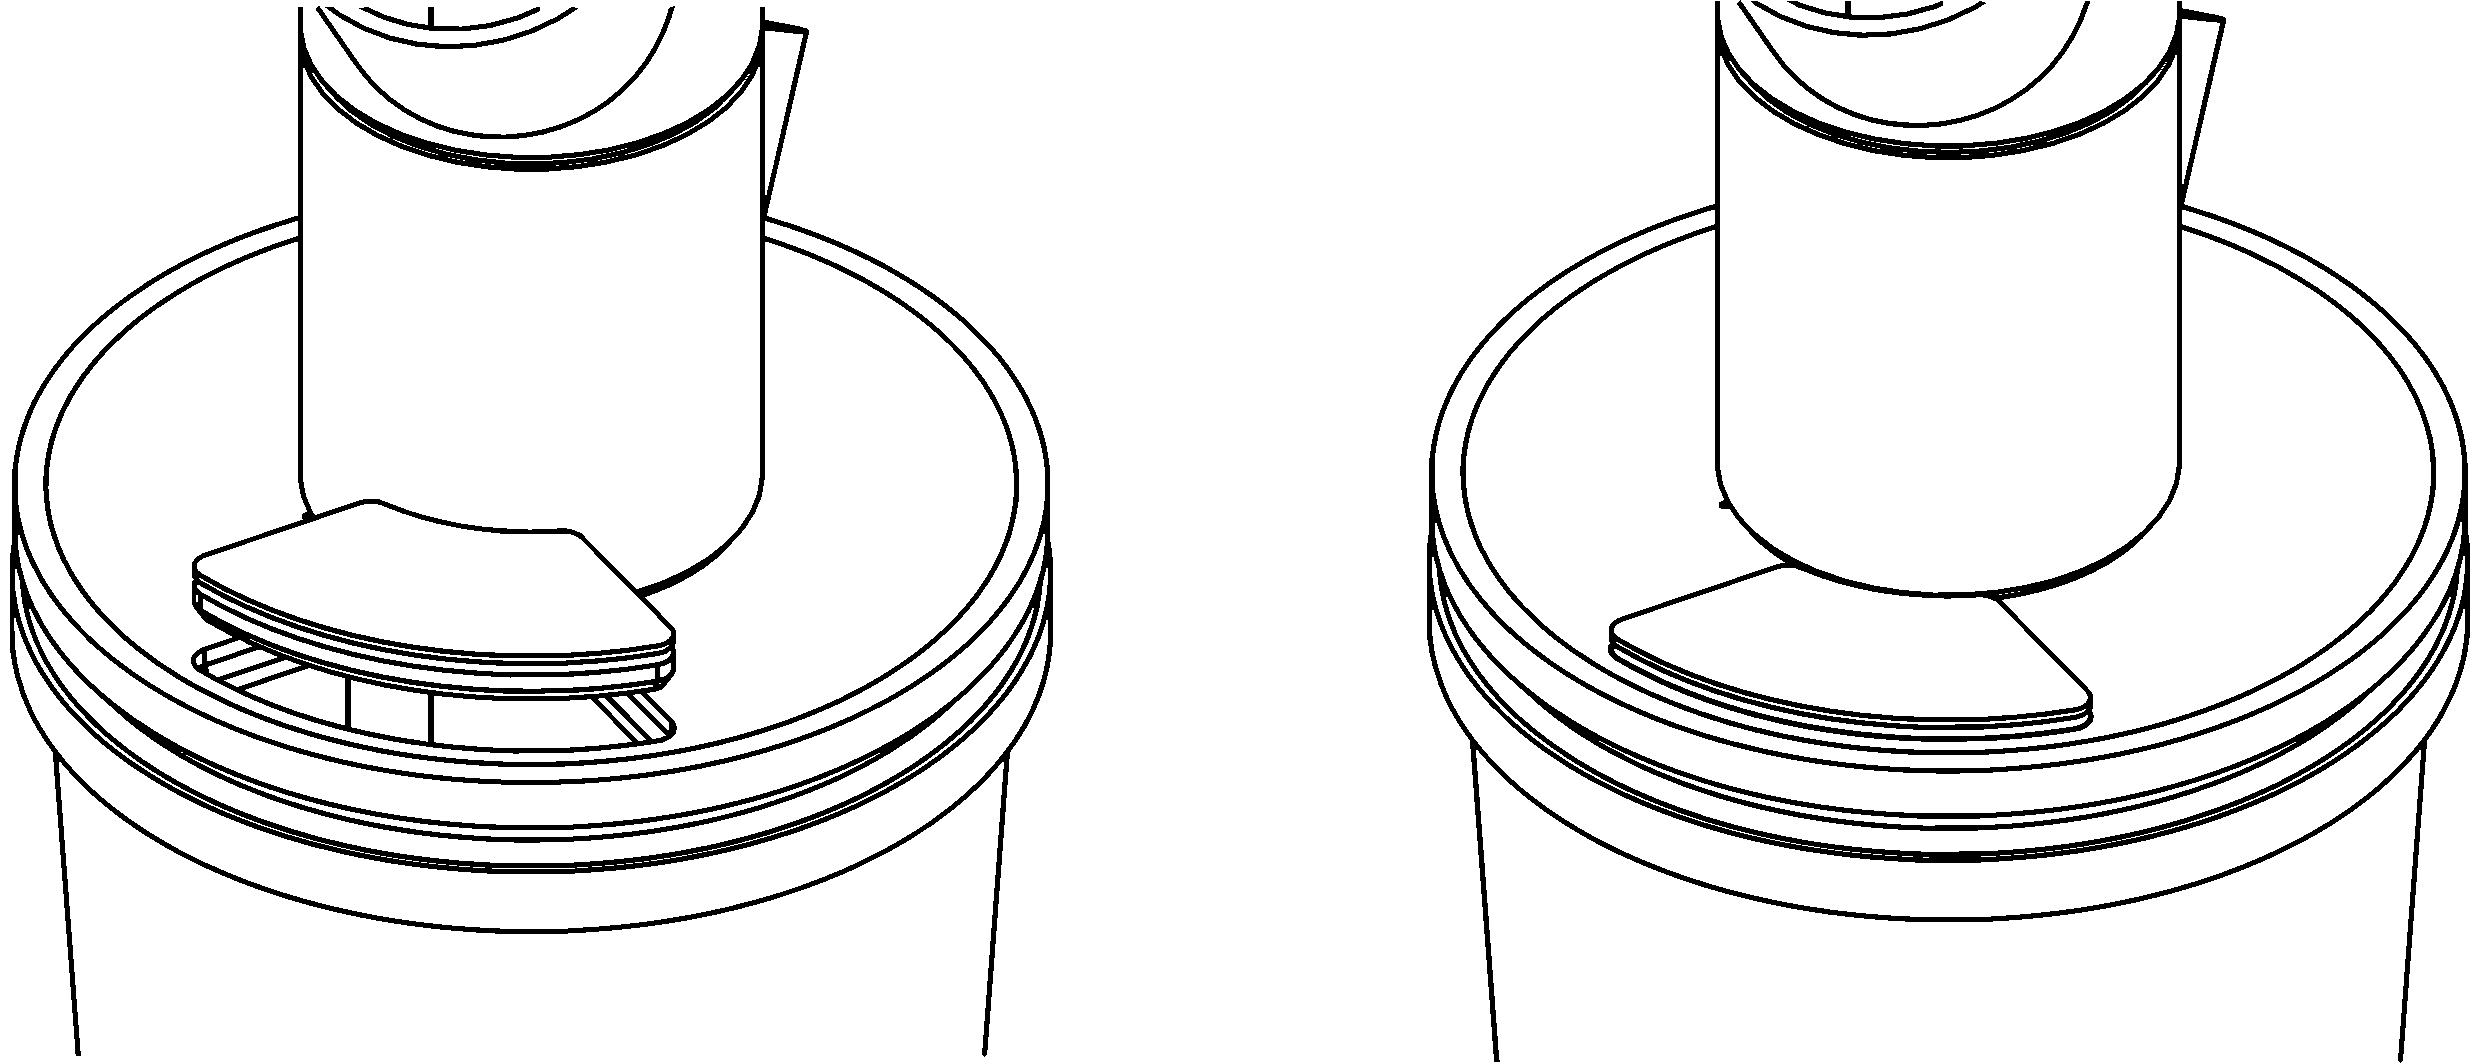
\includegraphics[width=0.8\textwidth]{images/80mm/80mm_assembly_10.png}
    \caption*{}
    \label{fig:80mm-ten}
\end{figure}
\begin{figure}[h]
    \centering
    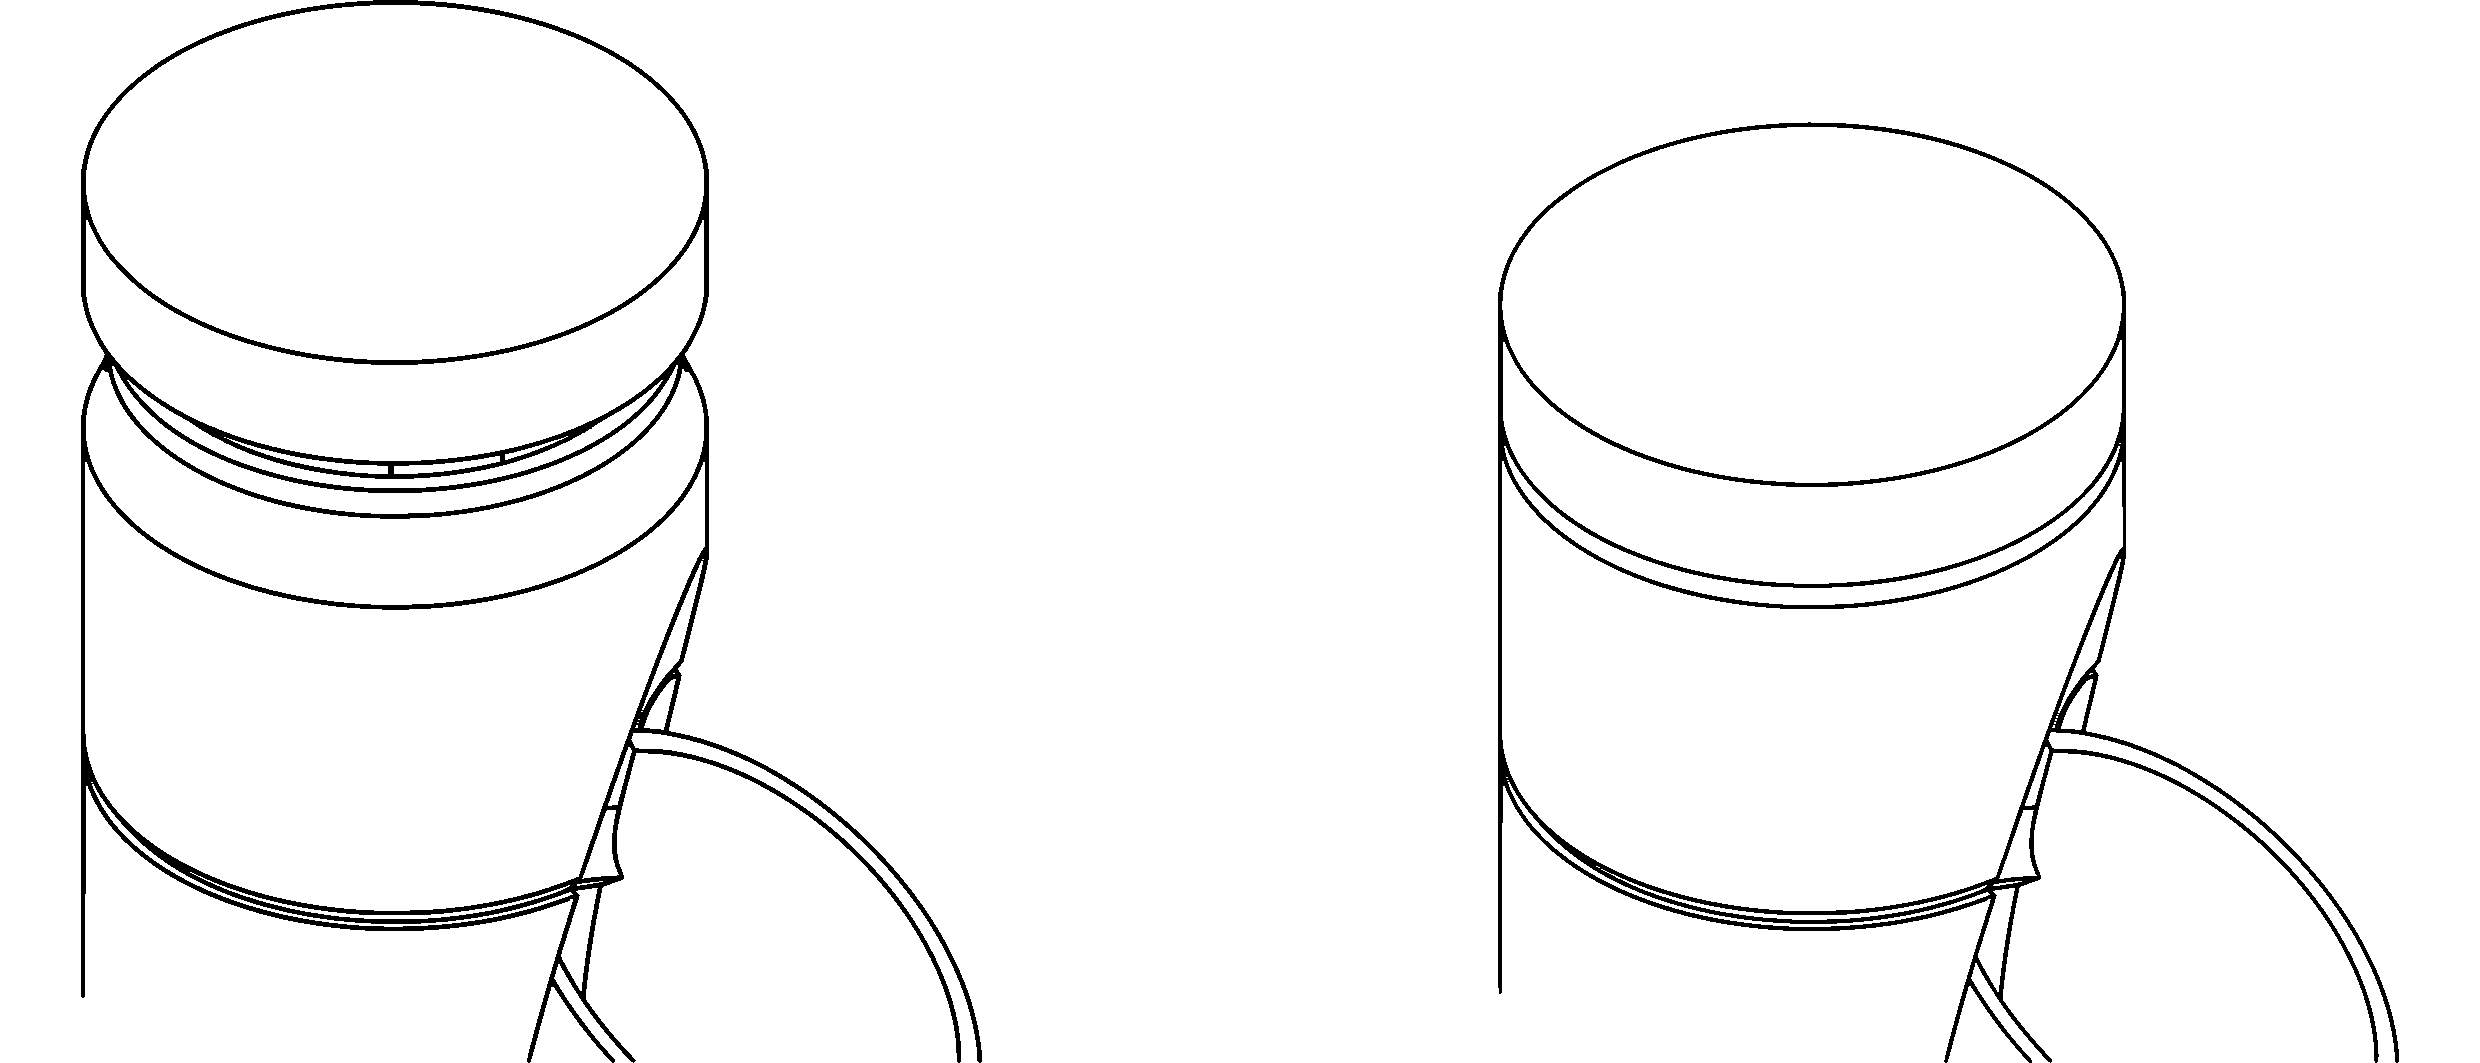
\includegraphics[width=0.8\textwidth]{images/80mm/80mm_assembly_11.png}
    \caption*{}
    \label{fig:80mm-eleven}
\end{figure}

\end{enumerate}

\setlength{\intextsep}{12.0pt plus 2.0pt minus 2.0pt}
\setlength{\floatsep}{12.0pt plus 2.0pt minus 2.0pt}
\setlength{\textfloatsep}{20.0pt plus 2.0pt minus 4.0pt}
\setlength{\belowcaptionskip}{0.0pt}


\clearpage

\section{Assembly Instructions -- 50mm}

\subsection{Parts}

\begin{center}
    \begin{minipage}{0.3\textwidth}
        \centering
        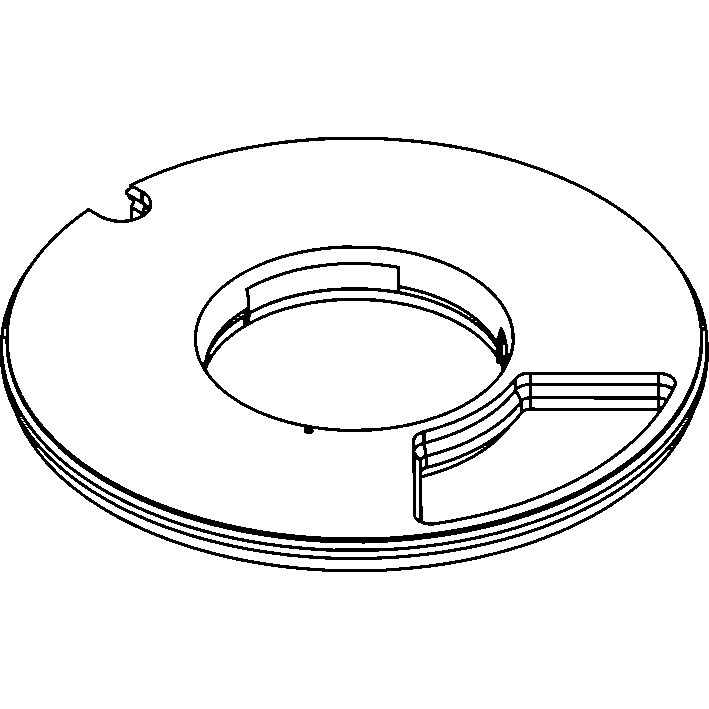
\includegraphics[height=3cm]{images/wireframes/bucket_lid.png}
        \captionof*{figure}{1x Bucket Lid}
    \end{minipage}
    \hfill
    \begin{minipage}{0.3\textwidth}
        \centering
        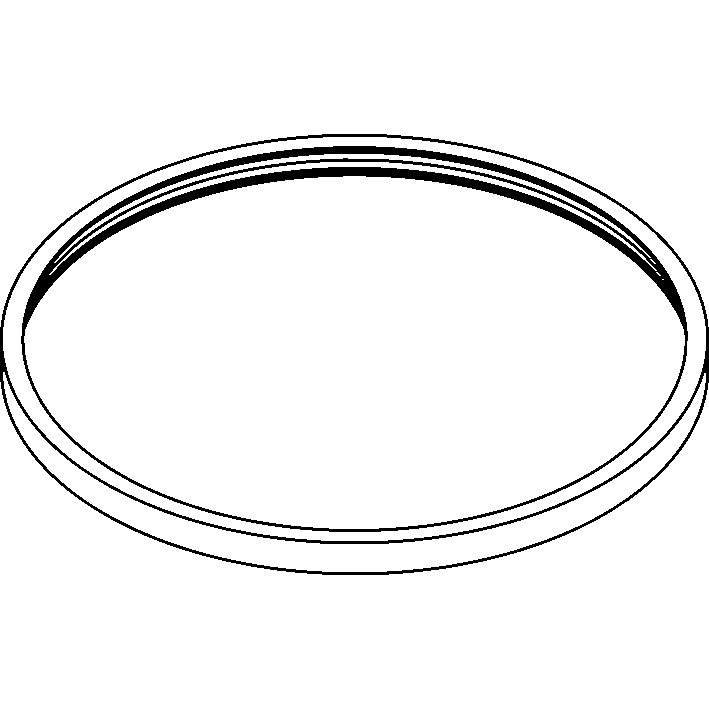
\includegraphics[height=3cm]{images/wireframes/bucket_lid_lockring.png}
        \captionof*{figure}{1x Bucket lid lock-ring}
    \end{minipage}
    \hfill
    \begin{minipage}{0.3\textwidth}
        \centering
        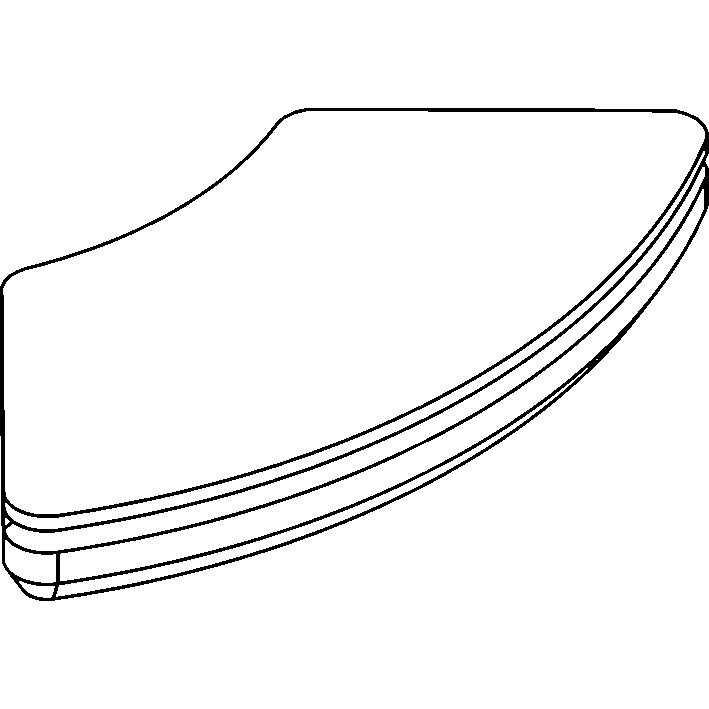
\includegraphics[height=3cm]{images/wireframes/bucket_lid_cap.png}
        \captionof*{figure}{1x Bucket lid cap}
    \end{minipage}

    \vspace{8pt}
    \rule{\textwidth}{0.5pt}
    \vspace{2pt}

    \begin{minipage}{0.3\textwidth}
        \centering
        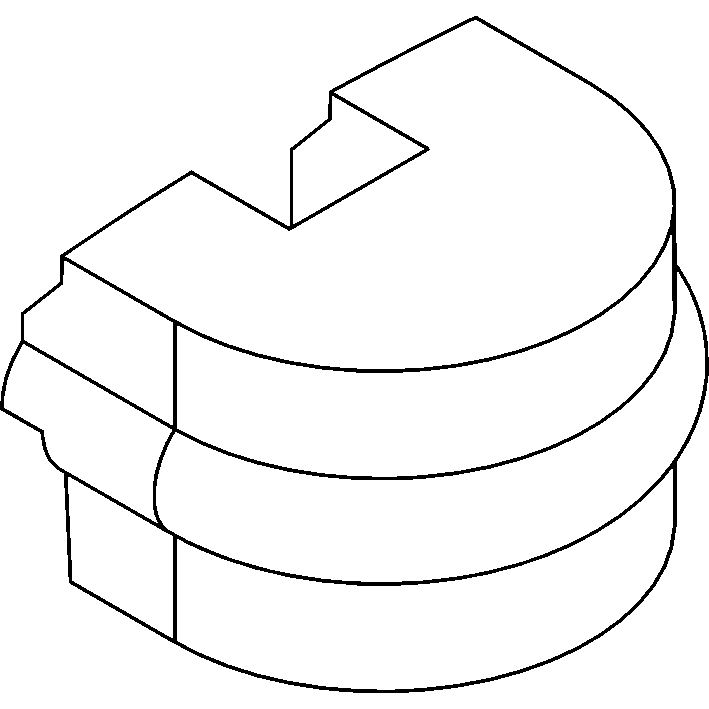
\includegraphics[height=3cm]{images/wireframes/cable_gland_2wire.png}
        \captionof*{figure}{1x Two-wire cable gland}
    \end{minipage}
    \hfill
    \begin{minipage}{0.3\textwidth}
        \centering
        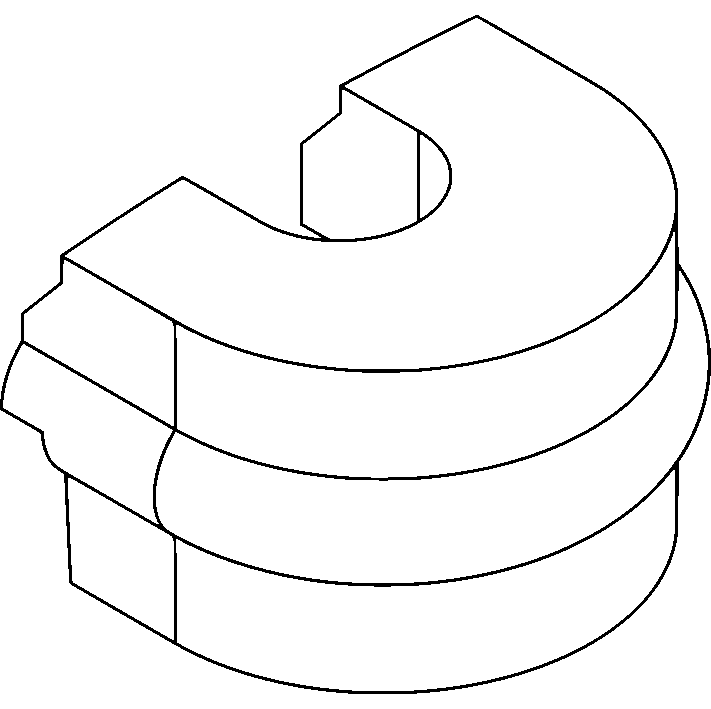
\includegraphics[height=3cm]{images/wireframes/cable_gland_3wire.png}
        \captionof*{figure}{1x Three-wire cable gland}
    \end{minipage}
    \hfill
    \begin{minipage}{0.3\textwidth}
        \centering
        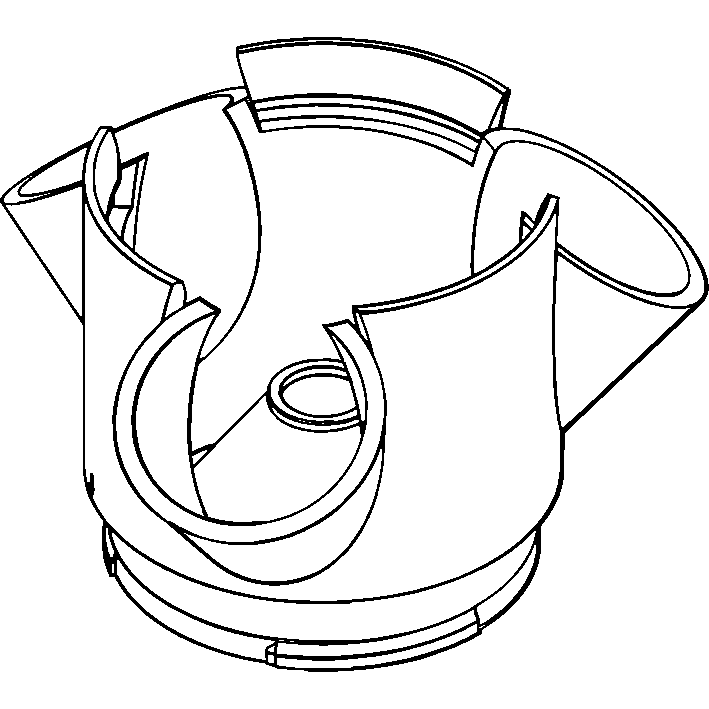
\includegraphics[height=3cm]{images/wireframes/50mm_base_module.png}
        \captionof*{figure}{1x Twist-lock base module}
    \end{minipage}

    \vspace{8pt}
    \rule{\textwidth}{0.5pt}
    \vspace{2pt}

    \begin{minipage}{0.3\textwidth}
        \centering
        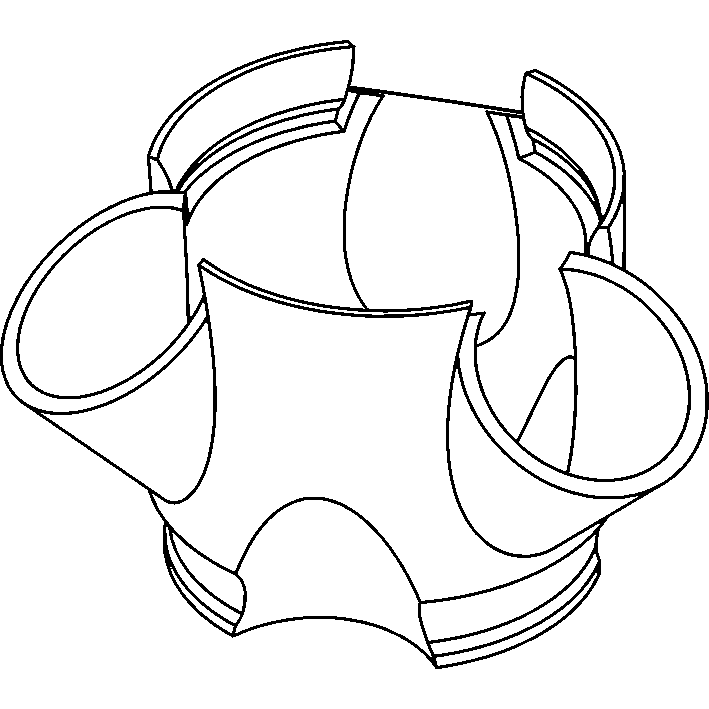
\includegraphics[height=3cm]{images/wireframes/50mm_module.png}
        \captionof*{figure}{5x Snap-fit module}
    \end{minipage}
    \hfill
    \begin{minipage}{0.3\textwidth}
        \centering
        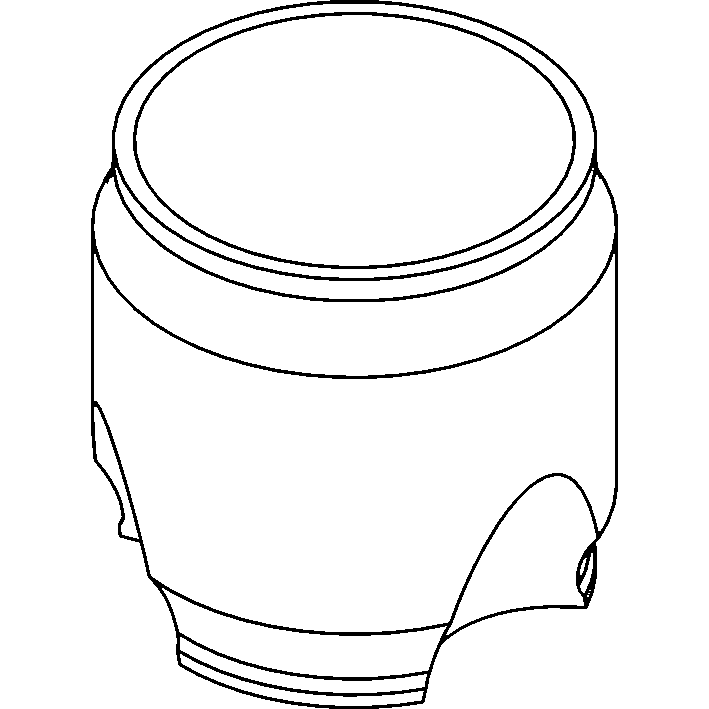
\includegraphics[height=3cm]{images/wireframes/50mm_chimney.png}
        \captionof*{figure}{1x Chimney module}
    \end{minipage}
    \hfill
    \begin{minipage}{0.3\textwidth}
        \centering
        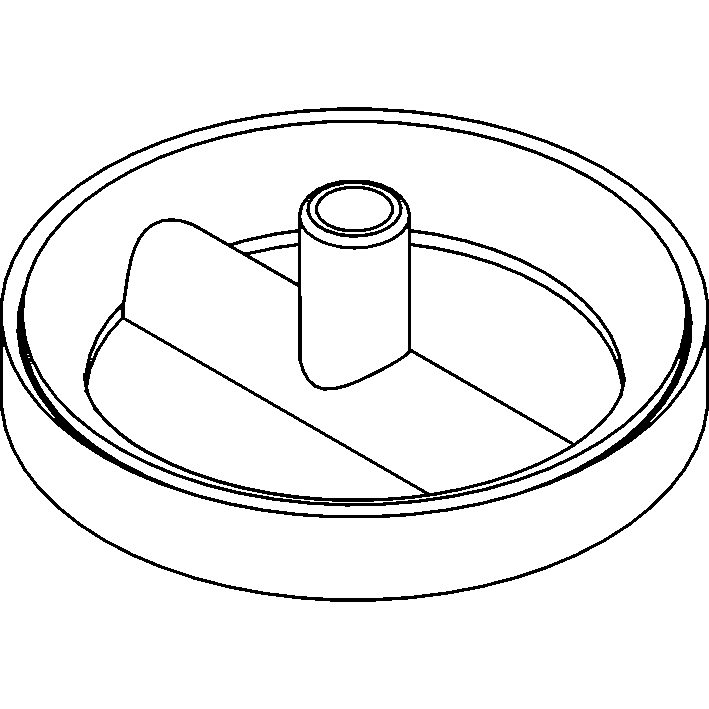
\includegraphics[height=3cm]{images/wireframes/50mm_shower_head.png}
        \captionof*{figure}{1x Shower head}
    \end{minipage}

    % \vspace{8pt}
    % \rule{\textwidth}{0.5pt}
    % \vspace{2pt}

    \begin{minipage}{0.3\textwidth}
        \centering
        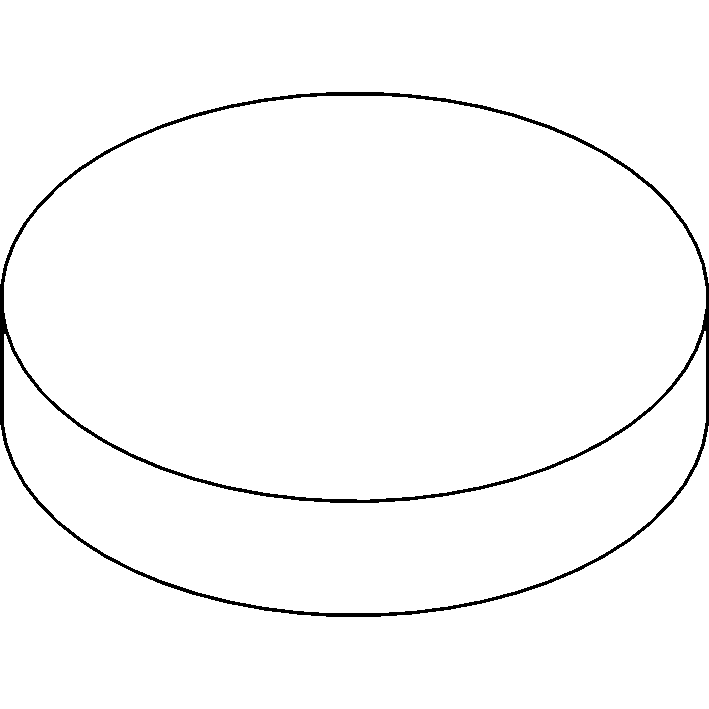
\includegraphics[height=3cm]{images/wireframes/chimney_lid.png}
        \captionof*{figure}{1x Chimney lid}
    \end{minipage}
    \hfill
    \begin{minipage}{0.3\textwidth}
        \centering
        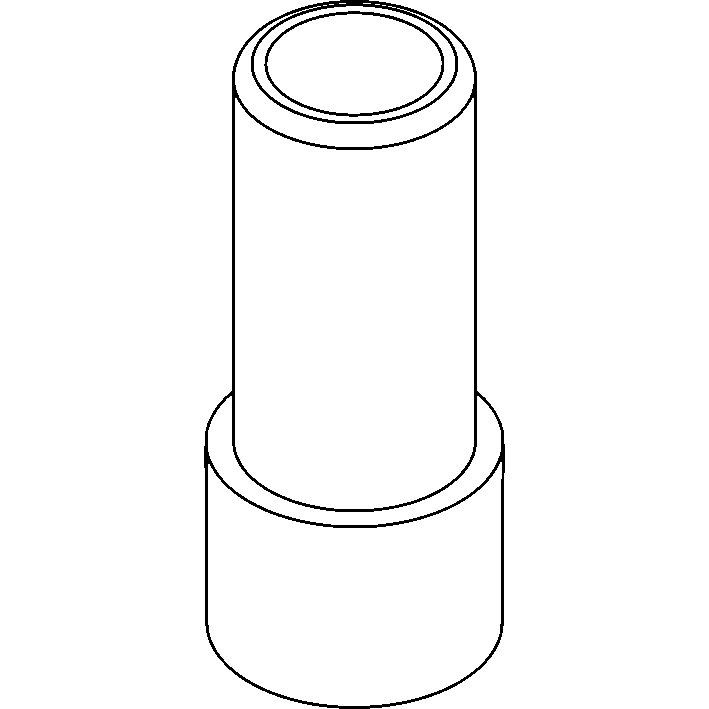
\includegraphics[height=3cm]{images/wireframes/adapter_13mm.png}
        \captionof*{figure}{1x 13mm hose adapter}
    \end{minipage}
    \hfill
    \begin{minipage}{0.3\textwidth}
        \centering
        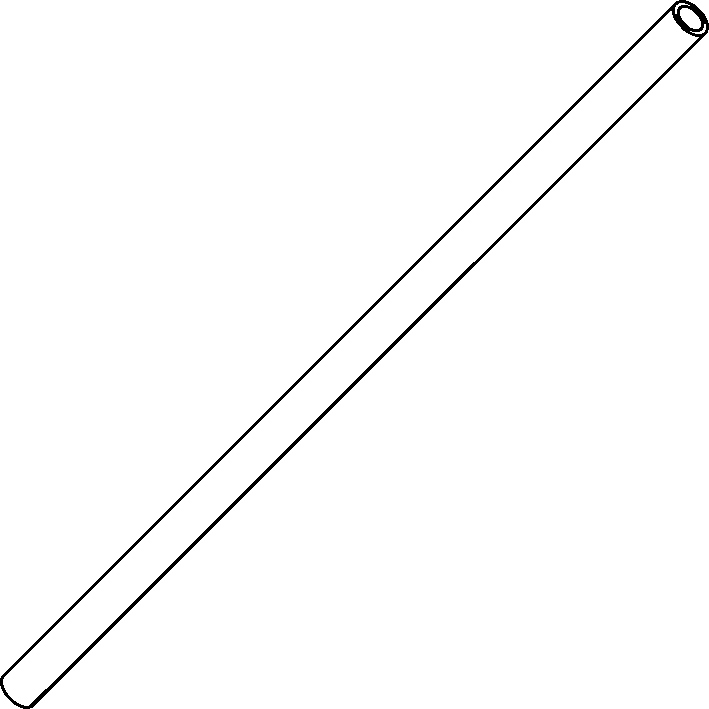
\includegraphics[height=3cm]{images/wireframes/hose_13mm.png}
        \captionof*{figure}{1x 13mm Hose}
    \end{minipage}

    \vspace{8pt}
    \rule{\textwidth}{0.5pt}
    \vspace{2pt}

    \begin{minipage}{0.3\textwidth}
        \centering
        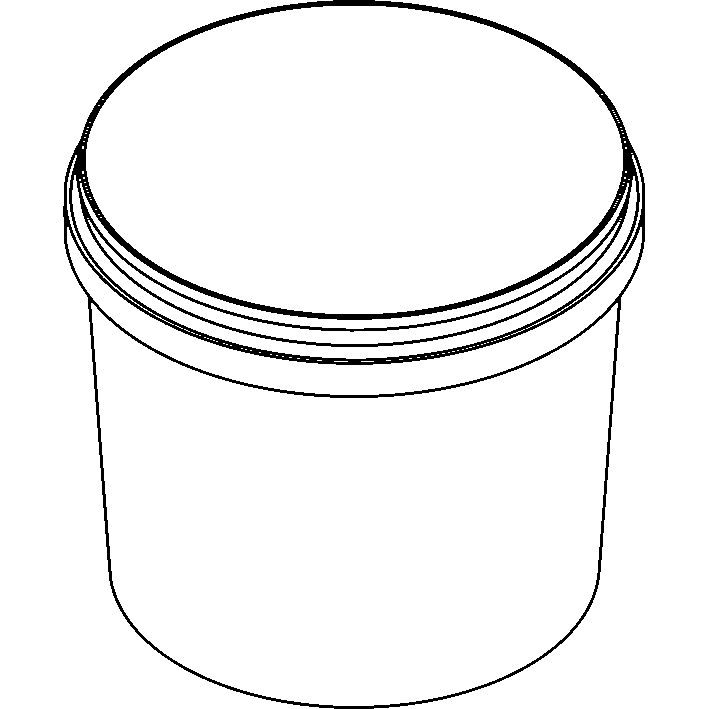
\includegraphics[height=3cm]{images/wireframes/bucket_5l.png}
        \captionof*{figure}{1x 5L Bucket}
    \end{minipage}
\end{center}

\clearpage

\setlength{\intextsep}{15.0pt plus 0.0pt minus 0.0pt}
\setlength{\floatsep}{10.0pt plus 0.0pt minus 0.0pt}
\setlength{\textfloatsep}{15.0pt plus 0.0pt minus 0.0pt}
\setlength{\belowcaptionskip}{-30.0pt}

\subsection{Assembly}

\begin{enumerate}

\item Align the arrow at the base of the \textbf{twist-lock base module} with the arrow on the top of the \textbf{bucket lid}. Carefully insert the base of the module into the hole in the center of the bucket lid when the arrows are aligned.

\item Once the \textbf{twist-lock base module} is inserted into the \textbf{bucket lid}, twist the module clockwise until you feel it stop. \textbf{Do not twist past this point.}

\begin{figure}[h]
    \centering
    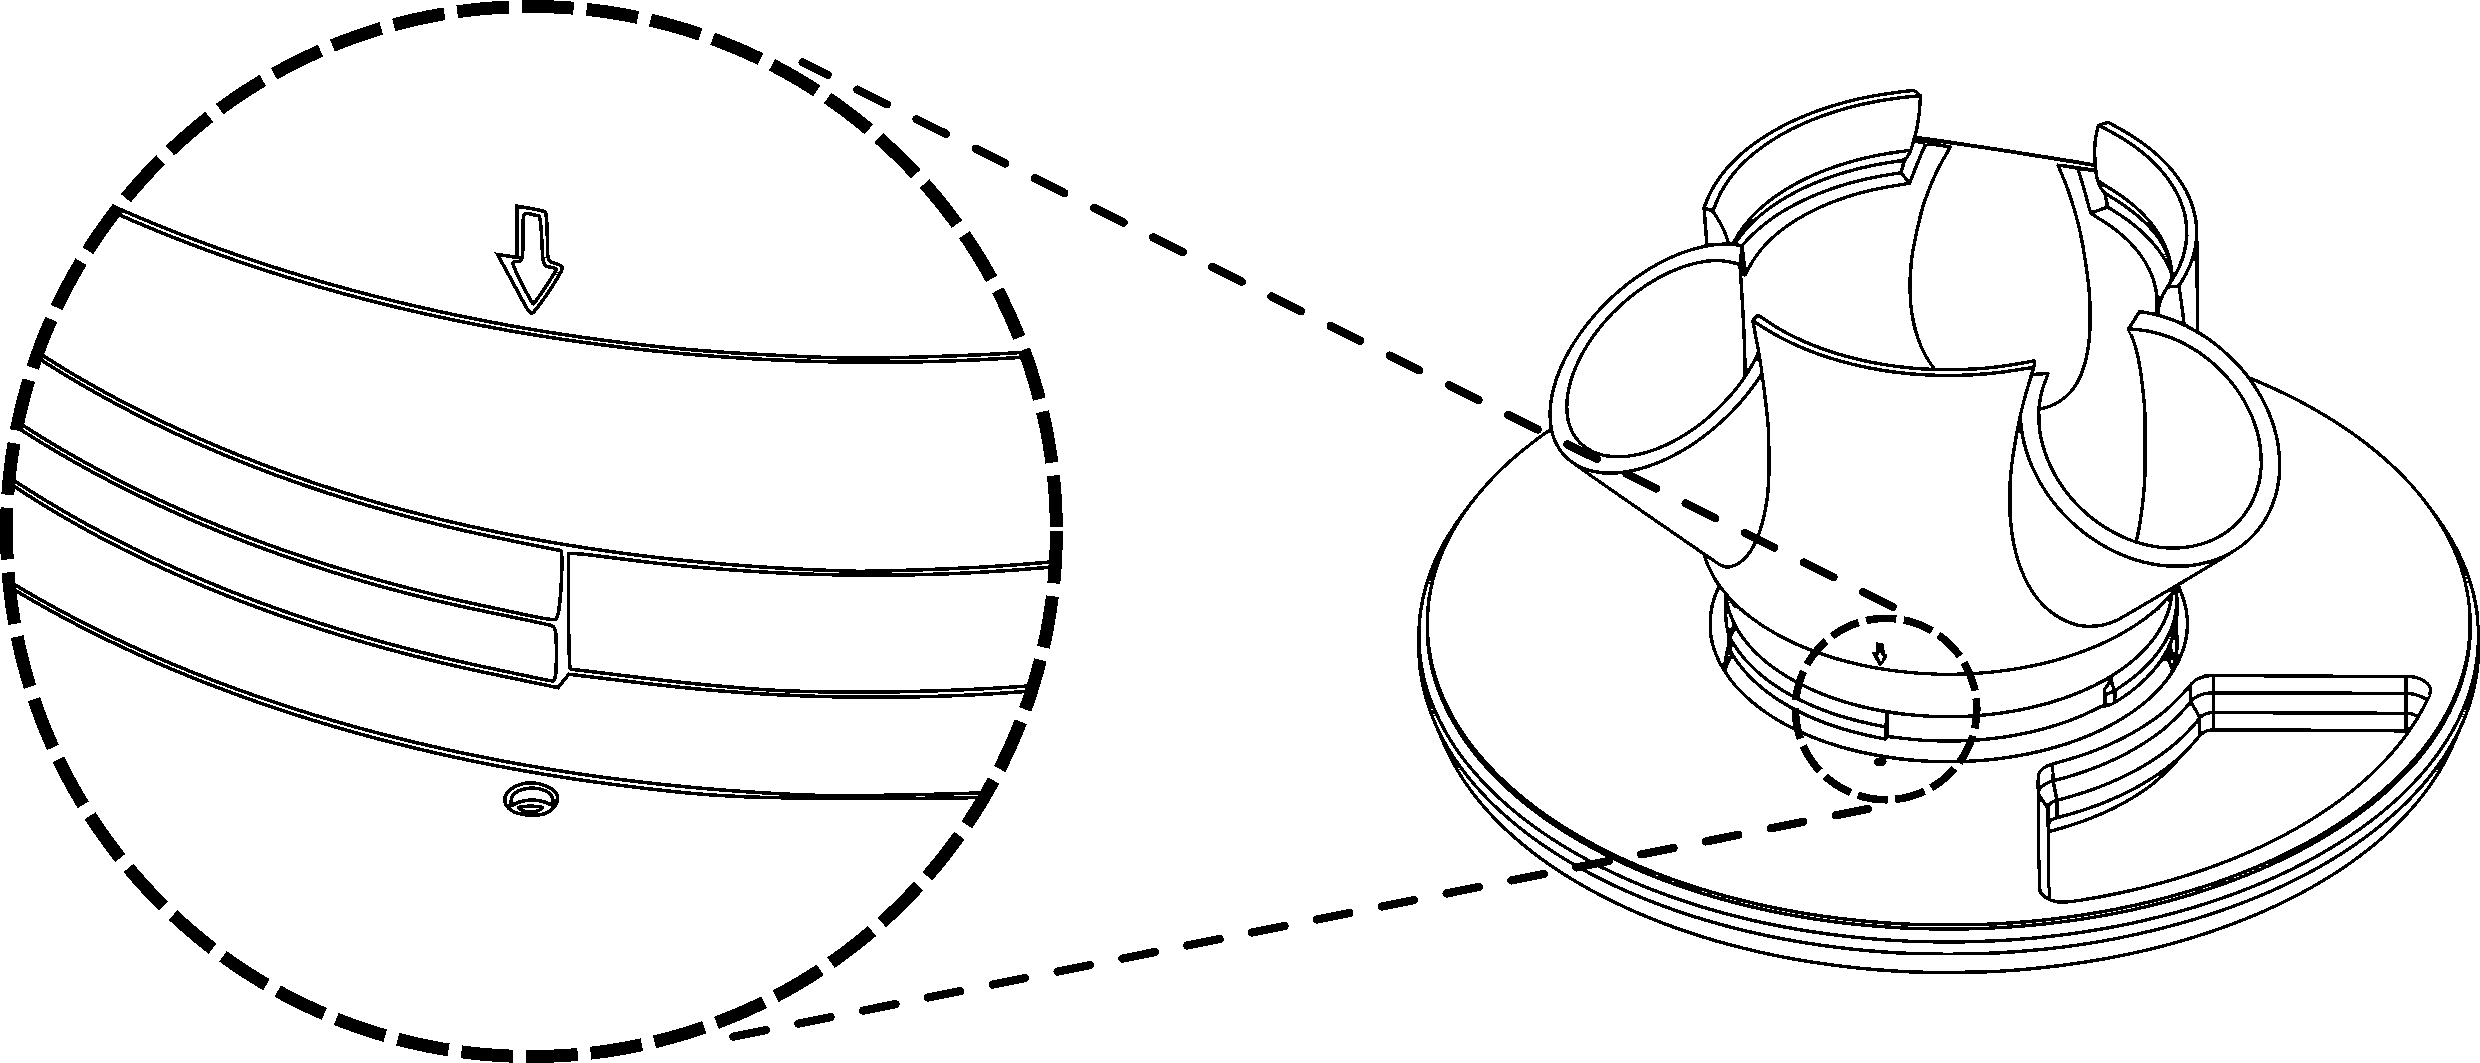
\includegraphics[width=0.8\textwidth]{images/50mm/50mm_assembly_1.png}
    \caption*{}
    \label{fig:50mm-one}
\end{figure}
\begin{figure}[h!]
    \centering
    
\includegraphics[width=0.8\textwidth]{images/50mm/50mm_assembly_2.png}
    \caption*{}
    \label{fig:50mm-two}
\end{figure}

\item Align the bottom of a \textbf{snap-fit module} with the top of the \textbf{twist-lock base module} so that the foot of the upper module fits into the receiver of the lower module, then gently push the upper module down until it snaps snugly together with the lower module.

\begin{figure}[h!]
    \centering
    
\includegraphics[width=0.8\textwidth]{images/50mm/50mm_assembly_3.png}
    \caption*{}
    \label{fig:50mm-three}
\end{figure}
\begin{figure}[h!]
    \centering
    
\includegraphics[width=0.8\textwidth]{images/50mm/50mm_assembly_4.png}
    \caption*{}
    \label{fig:50mm-four}
\end{figure}

\item Repeat step 3 with the remaining planter modules.

\item Using the same method, insert the \textbf{chimney module} into the snap-fit receiver of the topmost planter module.

\item Insert the water inlet of the \textbf{shower head} into one end of the \textbf{13mm hose}.

\begin{figure}[h!]
    \centering
    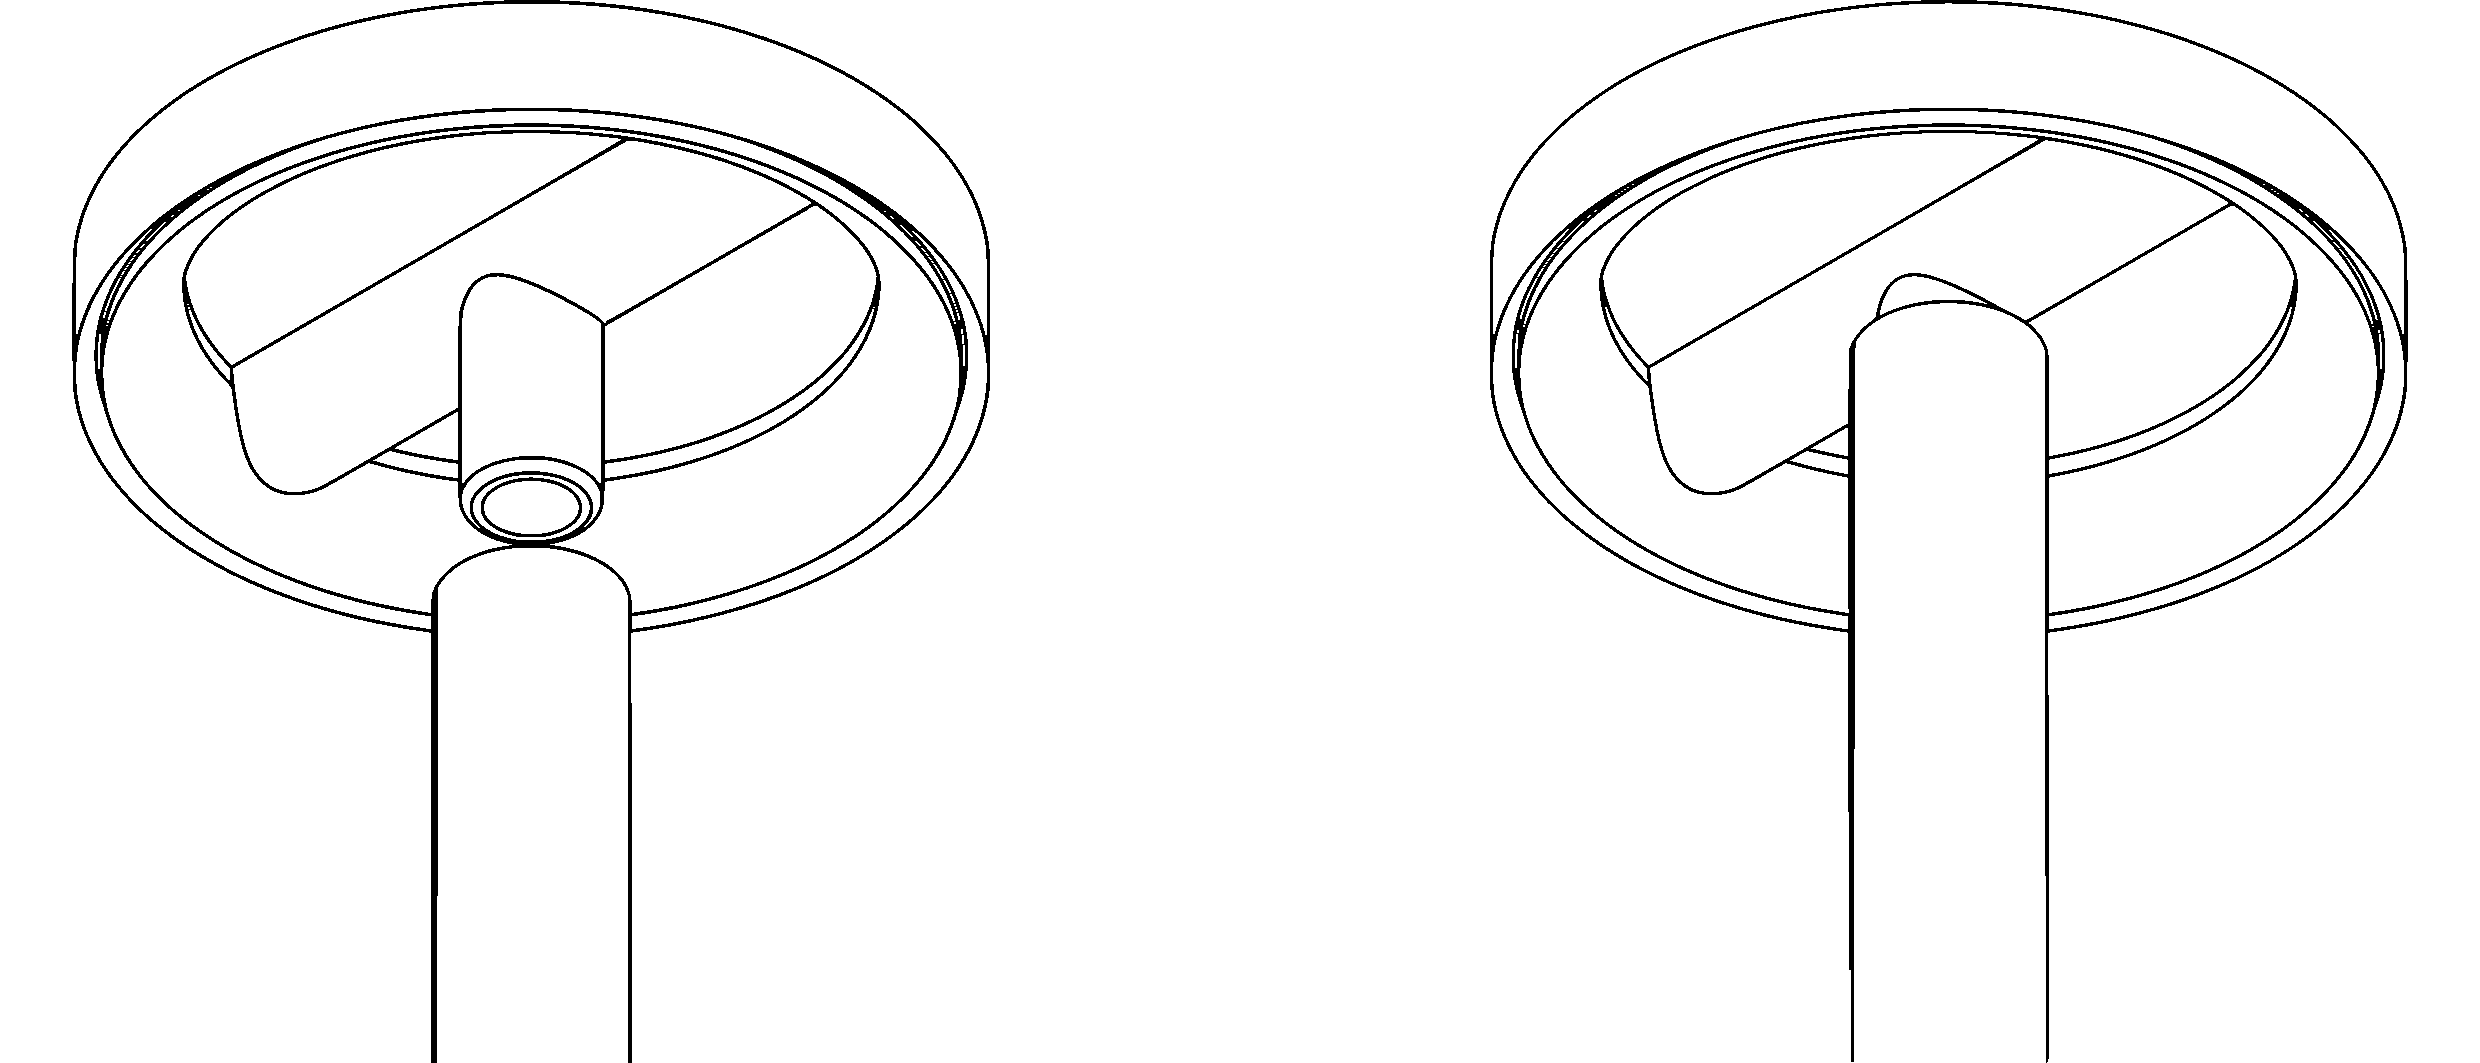
\includegraphics[width=0.8\textwidth]{images/50mm/50mm_assembly_5.png}
    \caption*{}
    \label{fig:50mm-five}
\end{figure}
\begin{figure}[h!]
    \centering
    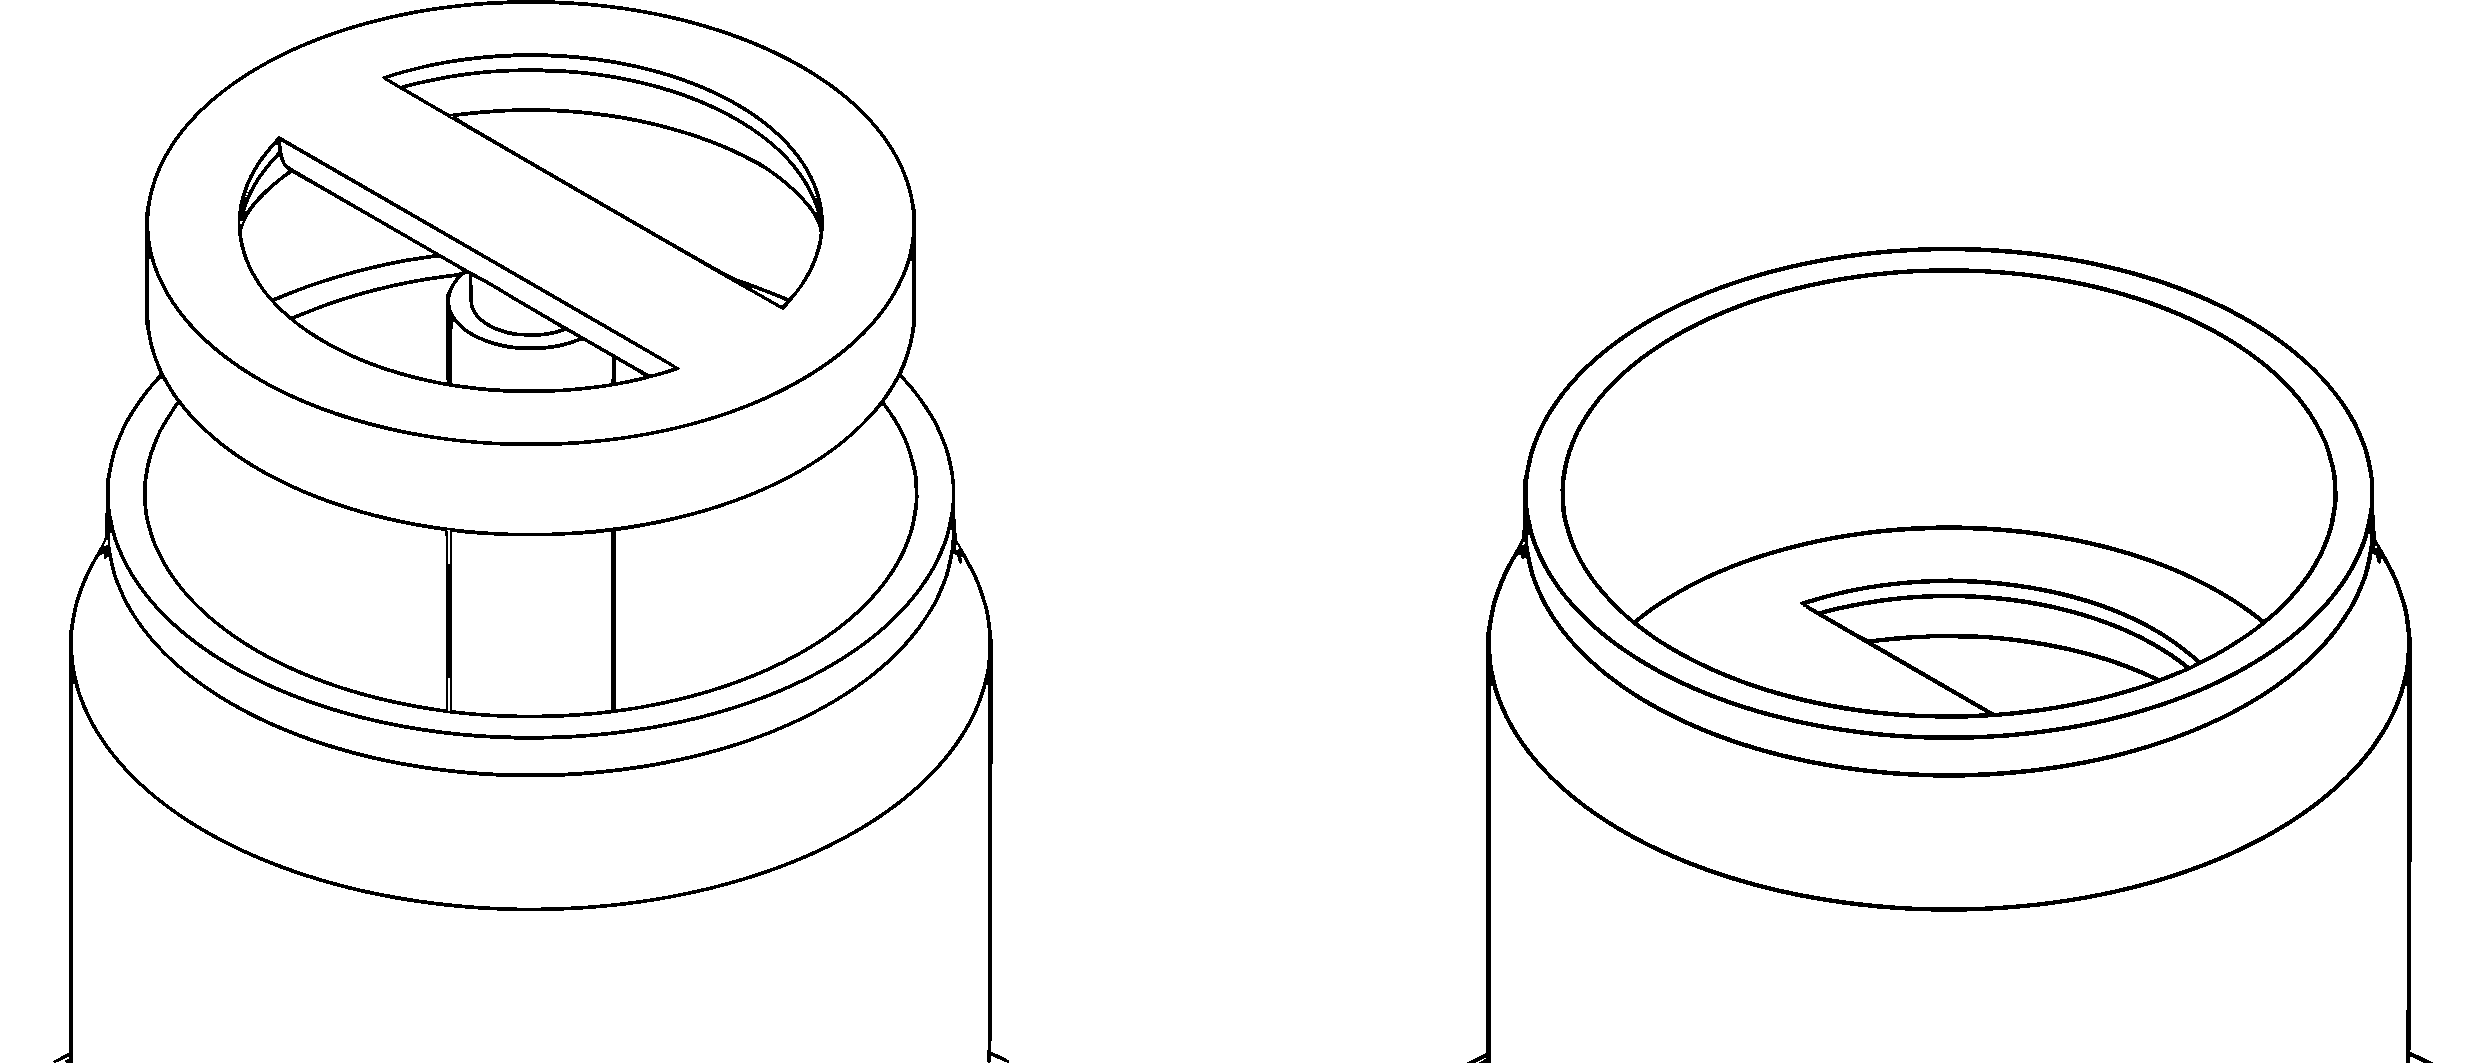
\includegraphics[width=0.8\textwidth]{images/50mm/50mm_assembly_6.png}
    \caption*{}
    \label{fig:50mm-six}
\end{figure}

\item Insert the opposite end of the \textbf{13mm hose} into the tower through the top of the \textbf{chimney module}, then insert the \textbf{shower head} into the top of the chimney module and push it down as far as it will go. Do not force the shower head further into the chimney module than it will go. The shower head is designed to fit snugly into the chimney module to aid the laminar flow of water over the inner wall of the tower, so \textbf{be careful not to angle the shower head as you insert it.}

\item Insert the appropriate \textbf{bucket lid cable gland} for your chosen pump's power cord into the cable gland receiver of the \textbf{bucket lid}. Be careful to ensure that the cable gland is oriented correctly, or the bucket lid won't sit properly on the bucket.

\begin{figure}[h!]
    \centering
    
\includegraphics[width=0.8\textwidth]{images/50mm/50mm_assembly_7.png}
    \caption*{}
    \label{fig:50mm-seven}
\end{figure}

\item Place your \textbf{submersible pump} in the \textbf{5L bucket}.

\item If using an Aqua One 103 pump or other Aqua One pump with the same outlet, insert the 13mm end of the \textbf{13mm hose adapter} into the free end of the 13mm hose. If using a different pump, appropriate adapters will need to be provided by the user.

\item While holding the tower so that the bucket lid hovers just above the lip of the bucket, connect the free end of the 13mm hose to the outlet of the submersible pump. You may need to adjust the position of the pump in the bucket to ensure that the pump outlet aligns with the hose.

\item Lower the bucket lid onto the lip of the bucket, ensuring that the power cord of the pump is routed through the bucket lid cable gland. As the bucket lid is lowered, gently pull the shower head upward inside the chimney so that the hose is straightened but not taut.

\item Lower the \textbf{bucket lid lock-ring}, with its flat side facing upward, down over the top of the tower. Align the lock-ring with the edge of the bucket lid, then carefully push the lock-ring down into place around the bucket-lid. It may be easiest to work from one point on the lock-ring and around to the other side in both directions simultaneously with both thumbs.

\item Insert the \textbf{bucket lid cap}, with its flat side facing upward, into the cap opening in the bucket lid.

\item Place the \textbf{chimney lid}, with its flat side facing upward, on top of the tower chimney.

\begin{figure}[h]
    \centering
    \vspace{-10pt}
    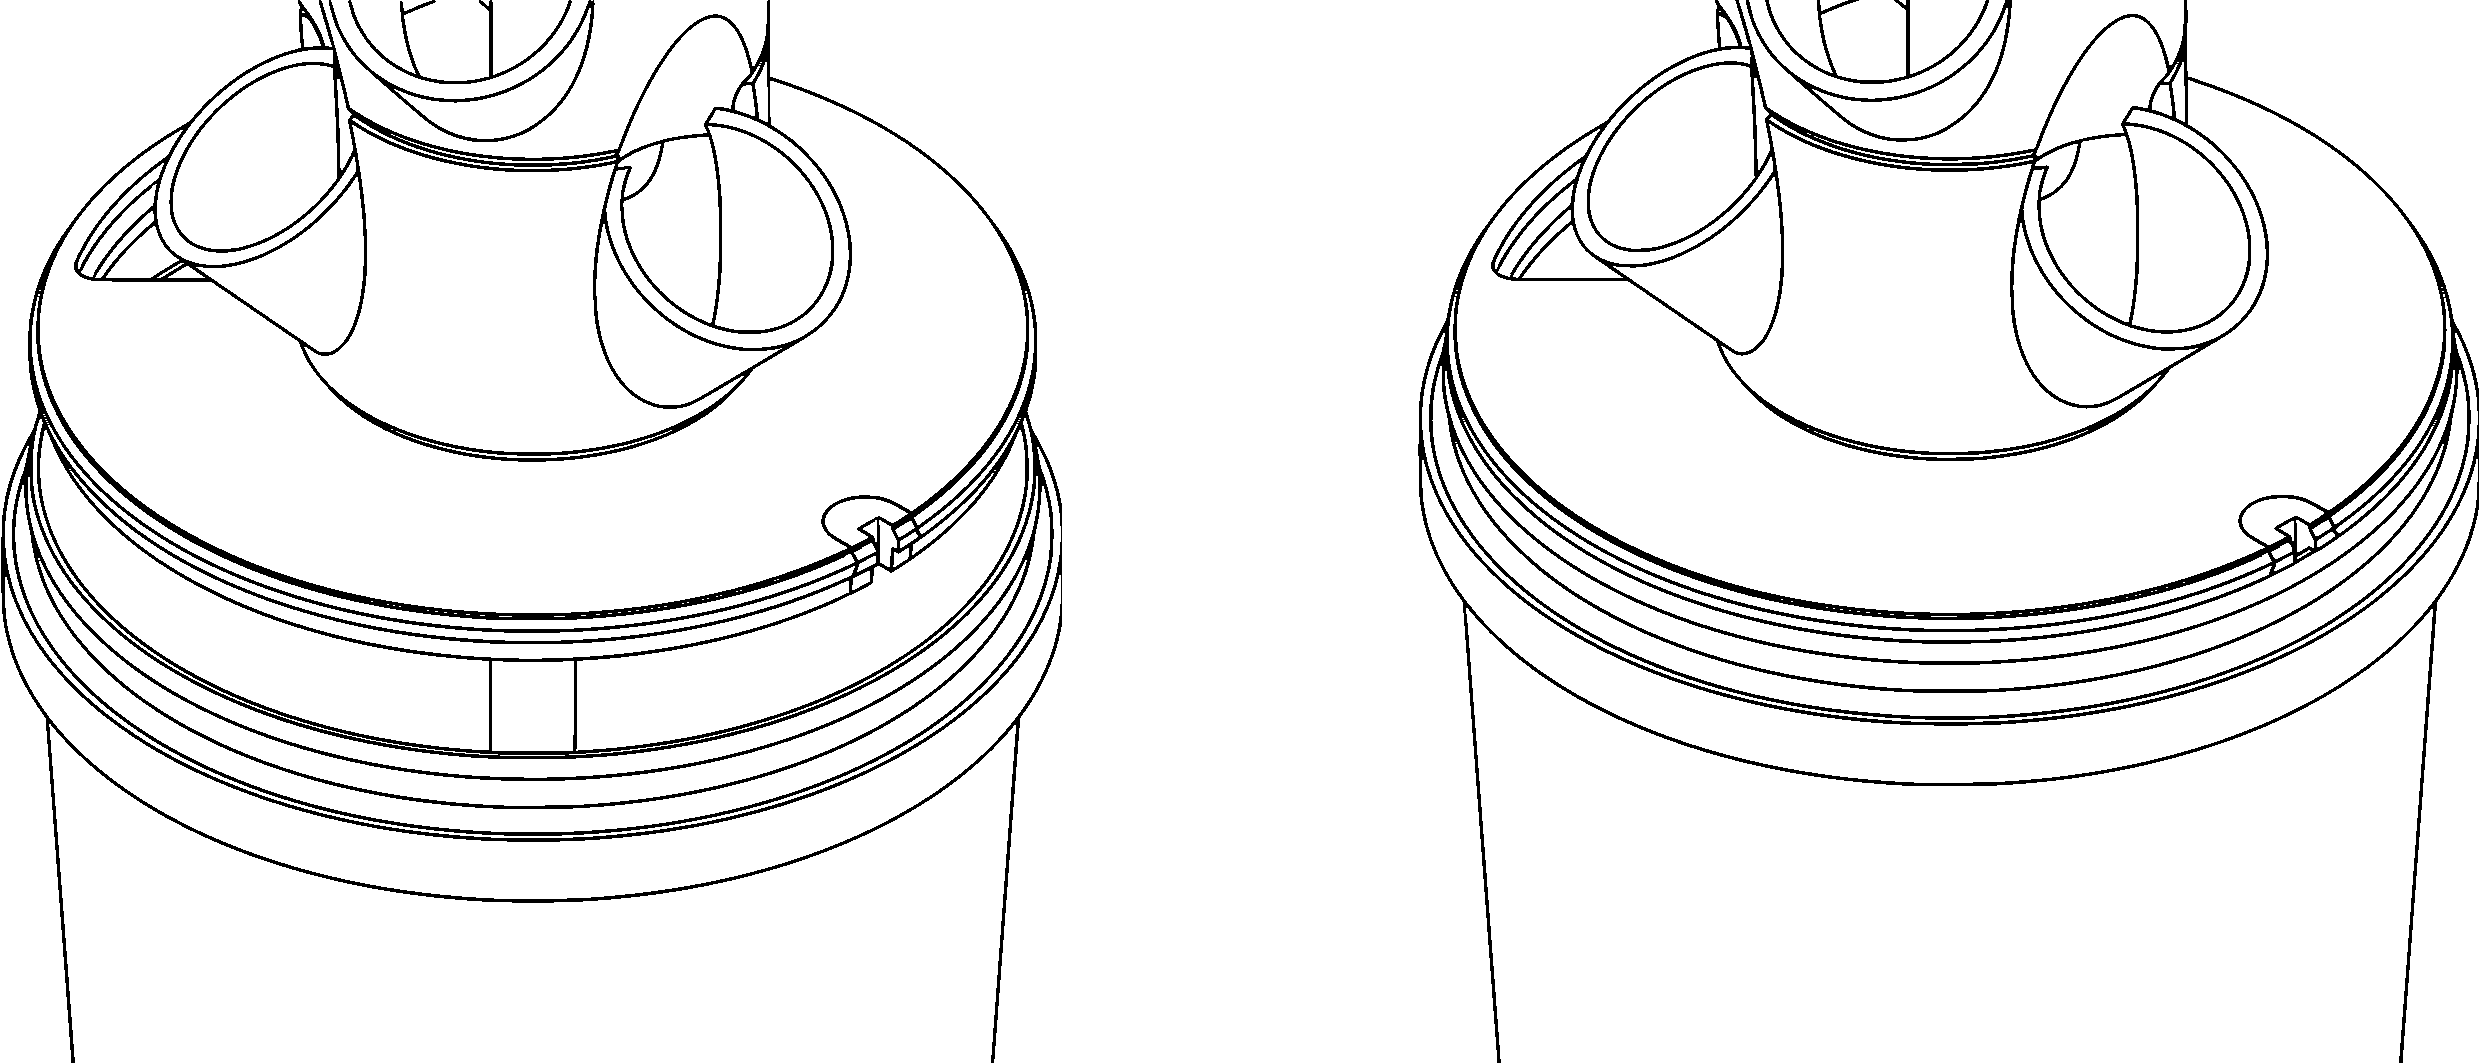
\includegraphics[width=0.8\textwidth]{images/50mm/50mm_assembly_8.png}
    \caption*{}
    \label{fig:50mm-eight}
\end{figure}

\begin{figure}[h]
    \centering
    
\includegraphics[width=0.8\textwidth]{images/50mm/50mm_assembly_9.png}
    \caption*{}
    \label{fig:50mm-nine}
\end{figure}
\begin{figure}[h]
    \centering
    
\includegraphics[width=0.8\textwidth]{images/50mm/50mm_assembly_10.png}
    \caption*{}
    \label{fig:50mm-ten}
\end{figure}
\begin{figure}[h!]
    \centering
    \includegraphics[width=0.8\textwidth]{images/50mm/50mm_assembly_11.png}
    \caption*{}
    \label{fig:50mm-eleven}
\end{figure}

\end{enumerate}

\setlength{\intextsep}{12.0pt plus 2.0pt minus 2.0pt}
\setlength{\floatsep}{12.0pt plus 2.0pt minus 2.0pt}
\setlength{\textfloatsep}{20.0pt plus 2.0pt minus 4.0pt}
\setlength{\belowcaptionskip}{0.0pt}


\clearpage

\section{Cleaning Suggestions}

\lipsum[1-3]


\end{document}
